\documentclass[10pt,letterpaper]{article}
\usepackage[top=0.85in,left=2.75in,footskip=0.75in,marginparwidth=2in]{geometry}

% use Unicode characters - try changing the option if you run into troubles with special characters (e.g. umlauts)
\usepackage[utf8]{inputenc}

% clean citations
\usepackage{cite}

% chemical formula
\usepackage{chemformula}

% SI units
\usepackage{siunitx}
\DeclareSIUnit{\molar}{M}

\usepackage{booktabs}

\usepackage{adjustbox}

% hyperref makes references clicky. use \url{www.example.com} or \href{www.example.com}{description} to add a clicky url
\usepackage{nameref,hyperref}

% line numbers
\usepackage[right]{lineno}

% improves typesetting in LaTeX
\usepackage{microtype}
\DisableLigatures[f]{encoding = *, family = * }

% text layout - change as needed
\raggedright
\setlength{\parindent}{0.5cm}
\textwidth 5.25in 
\textheight 8.75in

% use adjustwidth environment to exceed text width (see examples in text)
\usepackage{changepage}

% adjust caption style
\usepackage[aboveskip=1pt,labelfont=bf,labelsep=period,singlelinecheck=off]{caption}

% remove brackets from references
\makeatletter
\renewcommand{\@biblabel}[1]{\quad#1.}
\makeatother

% headrule, footrule and page numbers
\usepackage{lastpage,fancyhdr,graphicx}
\usepackage{epstopdf}
\pagestyle{myheadings}
\pagestyle{fancy}
\fancyhf{}
\rfoot{\thepage/\pageref{LastPage}}
\renewcommand{\footrule}{\hrule height 2pt \vspace{2mm}}
\fancyheadoffset[L]{2.25in}
\fancyfootoffset[L]{2.25in}

% use \textcolor{color}{text} for colored text (e.g. highlight to-do areas)
\usepackage{color}

% define custom colors (this one is for figure captions)
\definecolor{Gray}{gray}{.25}

% this is required to include graphics
\usepackage{graphicx}
\usepackage{subcaption}

% use if you want to put caption to the side of the figure - see example in text
\usepackage{sidecap}

% use for have text wrap around figures
\usepackage{wrapfig}
\usepackage[pscoord]{eso-pic}
\usepackage[fulladjust]{marginnote}
\reversemarginpar

% document begins here
\begin{document}
\vspace*{0.35in}

% title goes here:
\begin{flushleft}
{\Large
\textbf{\newline{Assessing Population Genetics Evidence for Local Adaptation to Phosphorus Availability in Maize.}
}
}
\bigskip
% authors go here:

\textbf{Doctoral Project Proposal} \\
Fausto Villafrade Rodríguez Zapata. M.Sc. 
\bigskip

\textbf{Thesis directors:} \\
Dr. Andrés Moreno Estrada.\\
Dr. Ruben Rellán Álvarez.

\bigskip
\textbf{Committee:}\\
Dr. Alexander de Luna \\
Dr. Luis Delaye Arredondo \\
Dr. Sean Michael Rovito  \\
Dr. Tania Hernández Hernández
\end{flushleft}

\section*{Abstract}
Plant phosphorus starving response (PSR) is a coordinated set of biochemical, physiological and developmental reactions to low phosphorus supply. I expect divergent selection in the loci involved in PSR if it is the result of local adaptation. Given the absence of opposing evolutionary forces, the main consequence of this selection is an increased frequency of adaptive alleles in populations exposed to low phosphorus availability. Here I use a reverse ecology approach to identify loci that might be involved in PSR and be subject to divergent selection. First I built soilP, an R package for assigning soil phosphorus retention potential to geographic locations. With this retention potential as phenotype I performed environmental GWAS on 3238 georeferenced landraces of \textit{Zea mays} from Latin America and the Caribbean. This resulted in the detection of significant signal from the 13 Mb span of \textit{Inv4m}, a previously reported adaptive retrogression from highland teosinte that includes \textit{ZmPho1;2a} an inorganic phosphate transporter. Finally, I propose analysis of phosphorus response in biparental populations polymorphic for \textit{Inv4m} in order to disentangle population structure from local adaptation or other environmental covariates.

% now start line numbers
\linenumbers

% the * after section prevents numbering
\section*{Introduction}

\paragraph{Phosphorus as limiting nutrient.} 
Different soil phosphorus compounds can be sorted into separate pools according their availability for direct plant use. The most readily available form for plants is Pi in aqueous solution. Next, is the phosphorus in organic compounds, such as nucleotides, phospholipids, phosphorylated sugars and proteins, from which phosphates can be hydrolyzed by enzymatic activity. After this, the non-occluded P fraction that corresponds to phosphate adsorbed to the surfaces of iron and aluminum oxides and \ch{CaCO3} \cite{walker1976}. One step less available is the occluded P fraction, that is, phosphate physically encapsulated or surrounded by secondary minerals, such as Fe, Al and Mn oxyhydroxides \cite{yang2013, filipelli2016} by coprecipitation or diffusive penetration \cite{walker1976}. Thus the labile, i.e. more bioavailable \cite{yang2013}, phosphorus pool includes phosphate ions in solution as well as P incorporated in soil organic matter, and to a lesser degree the non-occluded P fraction. The refractory forms, which are not easily bioavailable, include P in non-weathered apatite minerals and the ocludded P fraction \cite{filipelli2016}. 
In experimental conditions added normal or high Pi concentrations in nutrient solution range from \SI{15}{\micro\molar} to \SI{0.1}{\milli\molar}, depending on the subject species \cite{scheible2015}. However lower realized concentrations are expected given phosphate precipitation in presence of calcium ions, that are usually part of the solution. Pi concentrations 0.3 to \SI{5}{\micro\molar} in soil solution, could be considered low if they do not support optimal plant growth \cite{scheible2015,schachtman1998}. Unfertilized soils rarely release P fast enough to support the high growth rates of crop plant species \cite{schachtman1998}.

\paragraph{Phosphate Starving Response (PSR).} 
When confronted with Pi scarcity, plants present biochemical, physiological and developmental adjustments, collectively known as phosphate starving response , that can improve aquisition, reallocation, mobilization and, in general, phosphorus use efficiency \cite{scheible2015}. Pi starvation results in a shift in the developmental program that can increase the fitness of the plant \cite{peret2011}. There are maize landraces in the Mexican highlands that show PSR response in field conditions. In the Purhepecha Plateau, Michoacán \cite{bayuelo-jimenez2011,bayuelo-jimenez2014}, local maize landraces showed adaptation to a phosphorus deficient Andisol in traits such as root length, lateral root number, root hairs, and phosphorus use efficiency defined lower inhibition of shoot growth under low P. Cloned genes intevening in PSR and candidates from maize, sorghum and \textit{Arabidopsis} are reviewed in \cite{calderon-vazquez2011} with funtions such as phosphate ion transport, transcription factors, micro-rna regulation, and lipid metabolism.

\paragraph{Local Adaptation.} 
The classical experimental design to prove local adaptation is the reciprocal transplant. In this design, the strict criterion for local adaptation is that a population must have higher fitness at its native site than any other population introduced to that site \cite{savolainen2013}. Local adaptation results in higher fitness  of a population in a local environment, relative to populations coming from different habitats \cite{kawecki2004}. It is both the observed pattern and the process dependent on divergent selection, the allele frequency change in the populations in response to selection that varies geographically \cite{tiffin2014}. Evolutionary forces against local adaptation include gene flow, migration and  mutation, because  they act contrary to genetic differentiation of the populations. In contrast genetic drift causes differentiation in allele frequencies that is not necessarily adaptive, and is thus a confounding factor when studying the genetic basis of local adaptation \cite{kawecki2004}. 

\paragraph{Phosphorus Retention Potential Map.} Since the time of domestication, around 8700 B.P \cite{hastorf2009}, the adaptation of maize to local soil conditions has mostly taken place before the widespread adoption of industrial fertilizers. In contrast to the current high input crop system, where low phosphorus availability is readily supplemented, preindustrial fertilization practices were far less effective if existent. Therefore, with low or no added phosphates to soil, phosphorus retention potential must have been a an even more limiting parameter for plant growth in preindustrial times. In this work I used retention potential from the Global Phosphorus Retention Potential Map \cite{batjes2011} as an indicator of soil phosphorus availability instead of soil phosphorus content because datasets of estimated phosphorus content have serious data gaps in Latin America and the Caribbean and/or are likely to include modern fertilizer input \cite{shangguan2014, yang2013, harvestchoice2010, sanchez2003}. 
The base raster for this map is derived from the Digital Soil Map of the World (1:5 million scale) \cite{fao1974a, fao1995}, and has 10 km resolution with a total of 4320 x 1686 pixels. The raster value for each pixel encodes a map unit identifier. A raster attribute table links each map unit with probabilities for 8 possible soil units. The resulting map of the dominant, i.e. most probable, soil units can be seen in Figure \ref{fig1} (a). An additional table stores the physicochemical properties per soil unit, and a corresponding column for phosphorus retention potential class assigned by Batjes based upon soil unit pH and mineralogy. There are 4 possible values for this phosphorus retention potential class: low (Lo), moderate (Mo), high (Hi), very high(VH). Phosphorus retention potential class probabilities are then defined as the sum of soil unit probabilities per phosphorus retention class in each map unit \ref{fig1}. The resulting probabilities are binned according to its dominant class, i.e. 75-100 \%, 50-75 \% and 25-50 \%, in order to obtain a summary ordinal scale of phosphorus retention score (Figure \ref{fig1} (b)) that can be coded as a number from 1 to 15. 

\begin{figure}[!bh] %s state preferences regarding figure placement here

% use to correct figure counter if necessary
%\renewcommand{\thefigure}{2}
\centering

\begin{subfigure}[b]{\textwidth}
   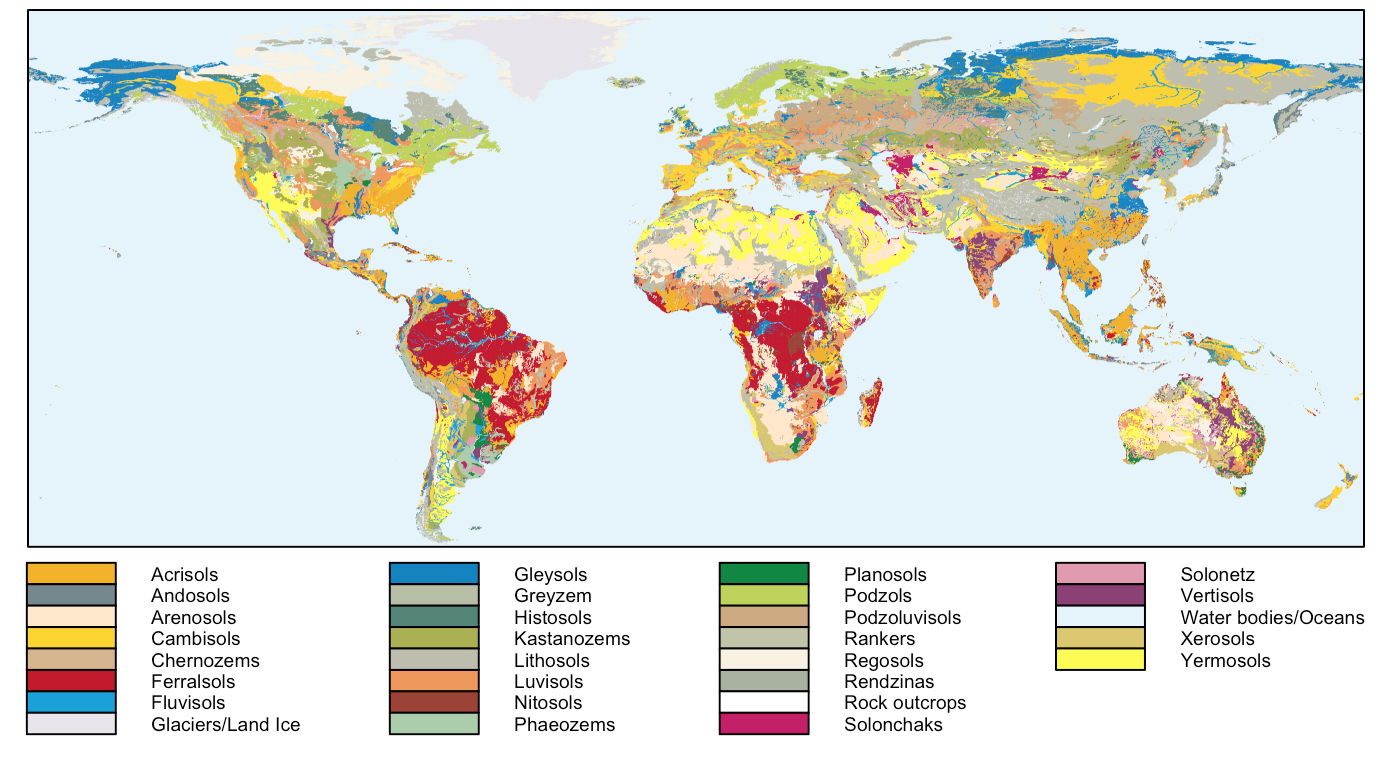
\includegraphics[width=0.9\linewidth]{fig1top.png}
   \label{fig0top} 
   \caption{\textbf{Digital Soil Map of the World}. Dominant soil groups \cite{fao1995} legend based upon \cite{faogis1999,fao1974a}.}
   \bigskip
\end{subfigure} 


\begin{subfigure}[b]{\textwidth}
   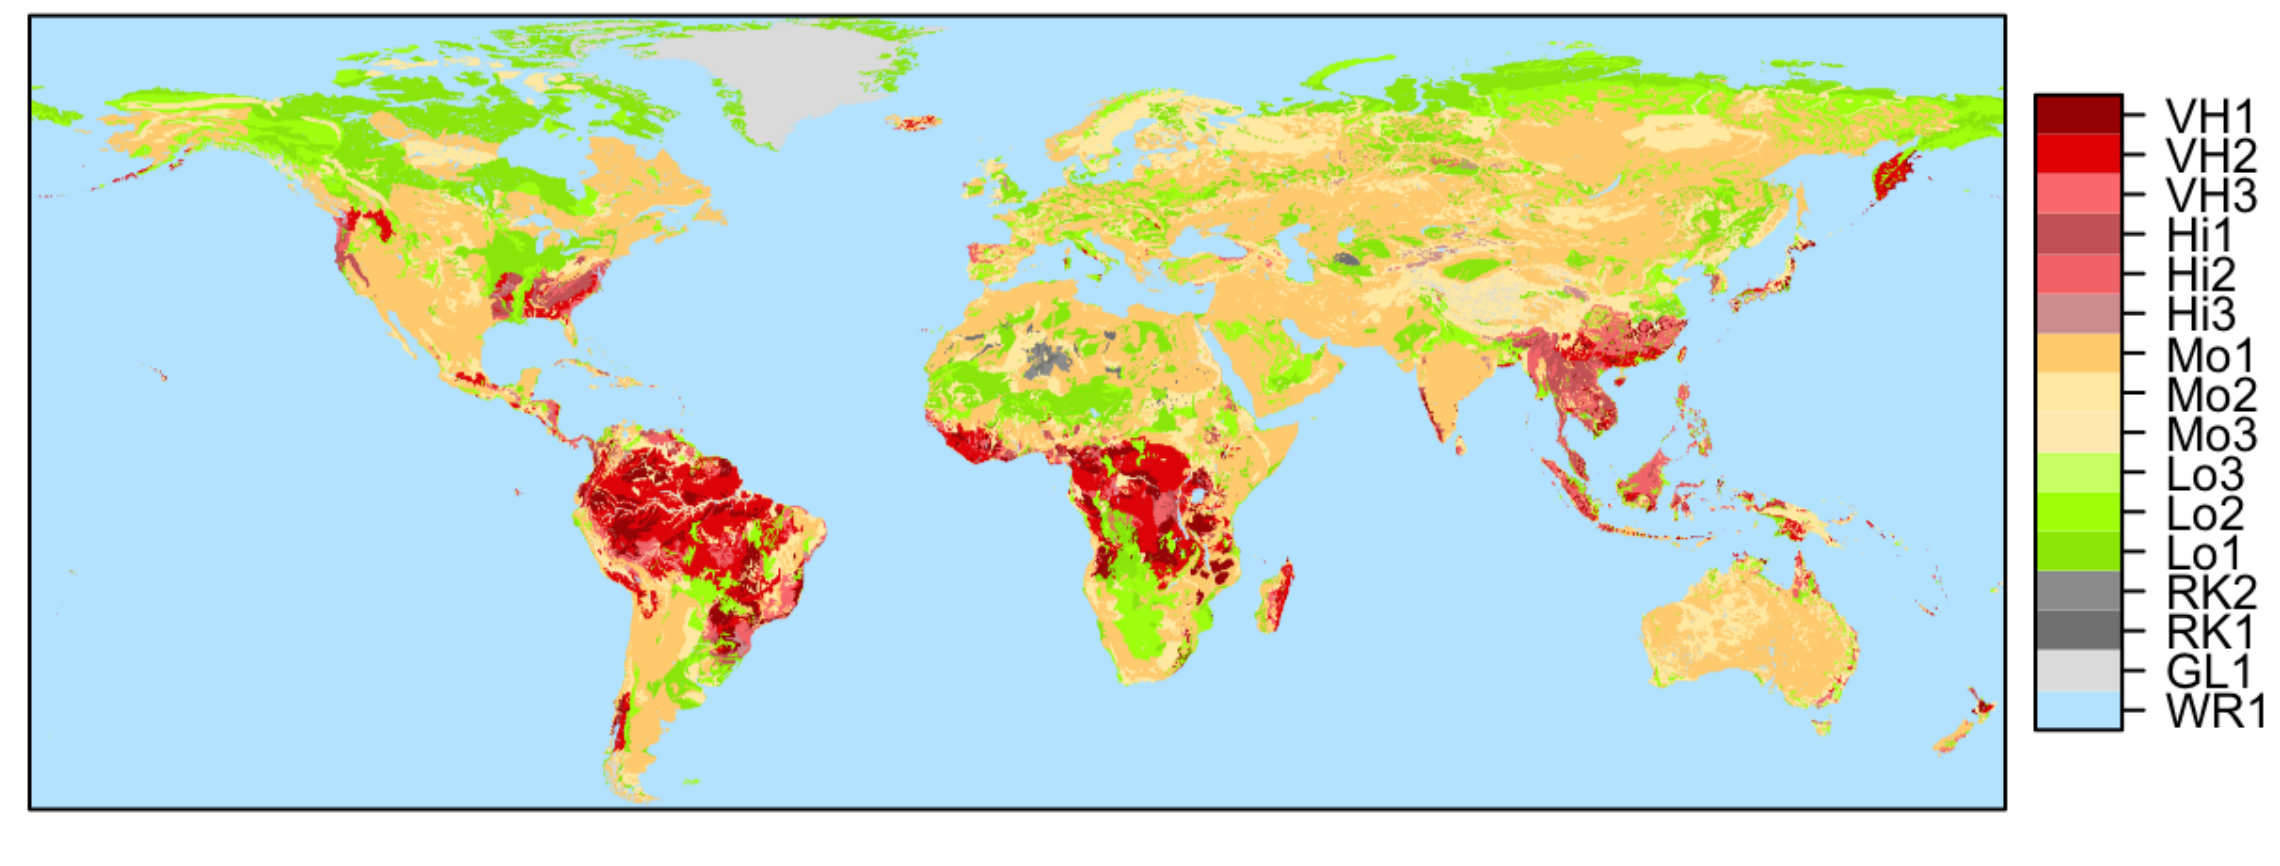
\includegraphics[width=1\linewidth]{fig1bottom.png}
   \label{fig0bottom} 
   \caption{\textbf{Global Phosphorus Retention Potential Map}. Retention classes are described by letters, VH: Very High; Hi: High; Mo: Moderate; Lo: Low; RK: Rock Outcrop; GL: Glacier; WR: Water. Class probability bins are represented by numerals, 1: 75-100 \%; 2: 50-75 \%; 3: 25-50 \%. Modified from \cite{batjes2011}.}
   \bigskip
\end{subfigure}


\caption{\textbf{Soil class defines phosphorus retention.}}
\label{fig1}

\end{figure}

\begin{figure}[htp] %s state preferences regarding figure placement here

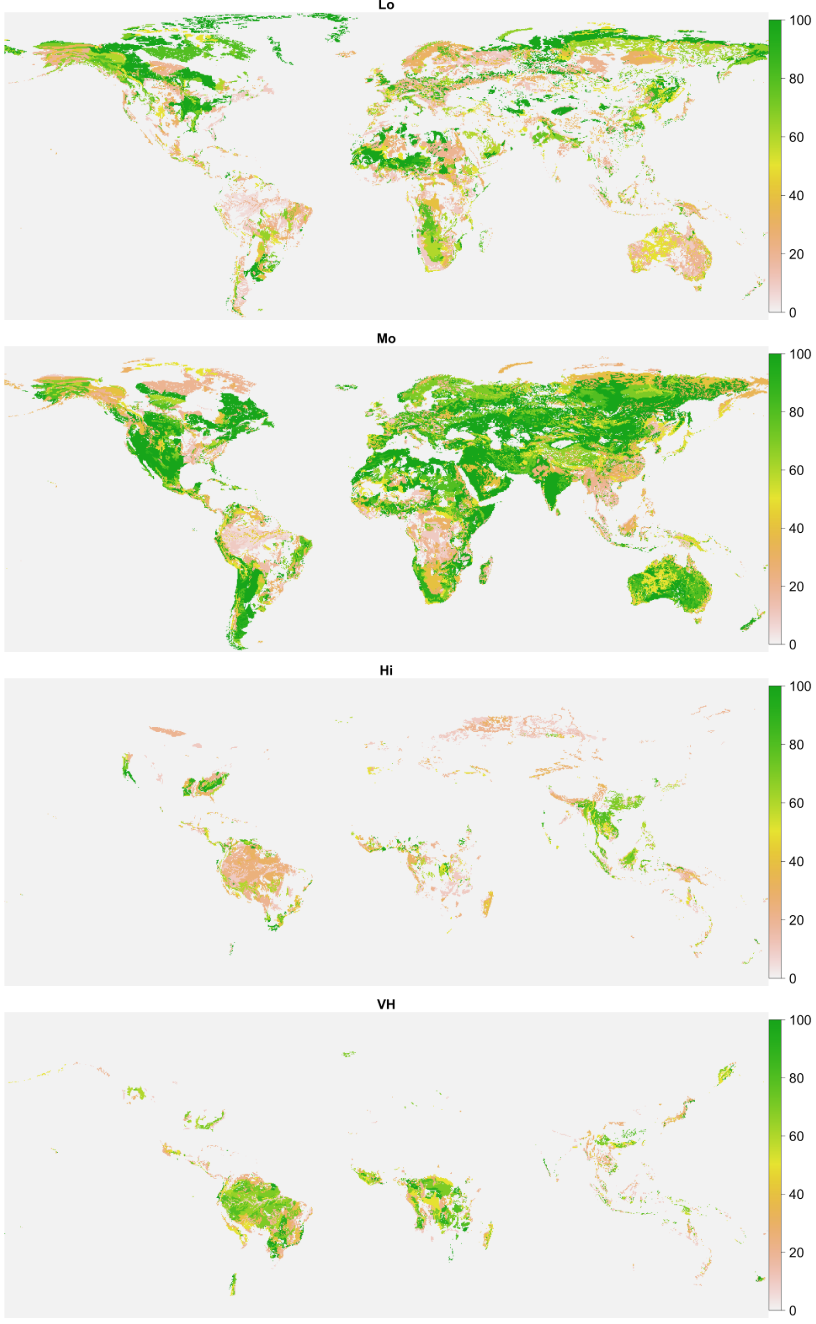
\includegraphics[width=\textwidth]{fig2.png}

\caption{\textbf{Soil Phosphorus Retention Class Probability Map.} Each channel represents one of the 4 retention classes, VH: Very High; Hi: High; Mo: Moderate; Lo: Low. The same data is summarized in Figure 2b. These probabilities were used as phenotypes for GWAS analysis on the maize landraces of \cite{romeronavarro2017}}

\label{fig2} % \label works only AFTER \caption within figure environment

\end{figure}

\section*{Objectives}

\paragraph{Main Goal} 

To assess the population genetics evidence for local adaptation to soil phosphorus availability in maize, and to dissect the genetic architecture of such adaptation.


\paragraph{Specific objectives}

\begin{enumerate}  
\item Find candidate loci for local adaptation using environmental GWAS in landrace populations.

\item Find evidence of selection in candidate loci between landrace populations.

\item Disentangle the confounding effects of environmental correlates and population structure through QTL analysis of phosphorus response in a biparental cross.
 
\end{enumerate}

\section*{Methods}
\subsection*{Environmental GWAS}

The GBS genotypes and geographic coordinates of 4711 maize landraces  from Latin America and the Caribbean  \cite{romeronavarro2017} are the base data for this work. I started from the set of biallelic imputed SNPs, B73 RefGen\_V2 as reference genome, having 1584871 markers. Then I selected  the 'GWAS dataset' as the 503016 markers with minor allele frequency greater than 0.01 in the 3238 georeferenced unrelated accessions (see below). 

The idea of a genome environment association is using environmental variables instead  of plant phenotypes as response variables \cite{lasky2015}. Here I use the soil phosphorus retention potential, both, as class probabilities and as summarizing scale from \cite{batjes2011}. With this aim I built \texttt{soilP} \cite{rodriguez-zapata2018}, an R package for extracting values from the Global Phosphorus Retention Potential Map and assigning them to arbitrary geographic locations. The soilP package and the detailed phosphorus variable extraction procedures are available at \url{https://github.com/sawers-rellan-labs/soilP}.

In addition to the phosphorus variables, I ran GWAS with selected environmental factors likely correlated to soil phosphorus retention potential. These comprise altitude and latitude \cite{romeronavarro2017}, topsoil pH, clay and sand content \cite{hengl2017}, and precipitation of the warmest quarter \cite{karger2017}. All environmental variables were extracted at the landrace coordinates from the corresponding 250 m or 1 km resolution geotiff using the R package \texttt{raster} for subsequent analysis \cite{hijmans2017,rcoreteam2018}

In order to correct for population structure I calculated the ancestry matrix $\mathbf{Q}$ for different number of postulated sub populations $K$ using the model based estimation from ADMIXTURE \cite{alexander2009}. However ADMIXTURE assumes that genotypes come from unrelated organisms and unlinked markers, hereafter named the 'structure dataset'. I decided to start the search for such a maximal independent set from a high quality matrix consisting of 6456 unimputed markers in 4511 individuals. Using \texttt{vcftools} \cite{danecek2011} I estimated both the plant relatedness coefficient $\phi$  according to the Manichaikul \cite{manichaikul2010} method,  and marker linkage disequibrium through $r^2$. This allowed me to use \texttt{fastindep} \cite{abraham2014} to arrive at a 'structure dataset' comprising 4368 unrelated plants at $\phi < \num{1e-6}$ and 4908 unlinked SNPs at $r^2 < 0.1$. Once this dataset fulfilled  ADMIXTURE's independence assumptions I estimated $\mathbf{Q}$ for $K = \{1 \ldots 50\}$ using its unsupervised method. Instead of using the Evanno $\Delta K$ method \cite{evanno2005}  for estimating the optimal number of subpopulations $K$ I used  ADMIXTURE's cross-validation criterion that requires less computational effort as it replaces complete dataset runs with runs of partially masked data (folds) \cite{alexander2009,lawson2018}. In this way I found  28 to be the optimal $K$, minimizing the cross validation error calculated from 5 fold runs \ref{figCV}. Then through ADMIXTURE's supervised method I projected the resulting ancestry on the individuals excluded from the 'structure dataset' for $K = \{3,10,28\}$  spanning a range up to the maximum reasonable $K$. After estimating ancestry for all the original 4711 landraces I finnally subsetted the $\mathbf{Q}$ matrix corresponding to the georeferenced unrelated common variants or 'GWAS dataset'. 

I ran the association studies as GLM models for each environmental variable  dependent on landrace genotypes with command line TASSEL 5 \cite{bradbury2007} using custom made shell scripts. As I constructed the 'GWAS dataset' from unrelated individuals I had no need for correcting the GLM model with a kinship matrix $\mathbf{K}$. However I did correct for $\mathbf{\{Q0, Q3, Q10, Q28\}}$ corresponding to no correction, and correction given the selected subpopulation numbers $K = \{3,10,28\}$ Figure \ref{fig6} (a-c).

\begin{figure}[!h]
   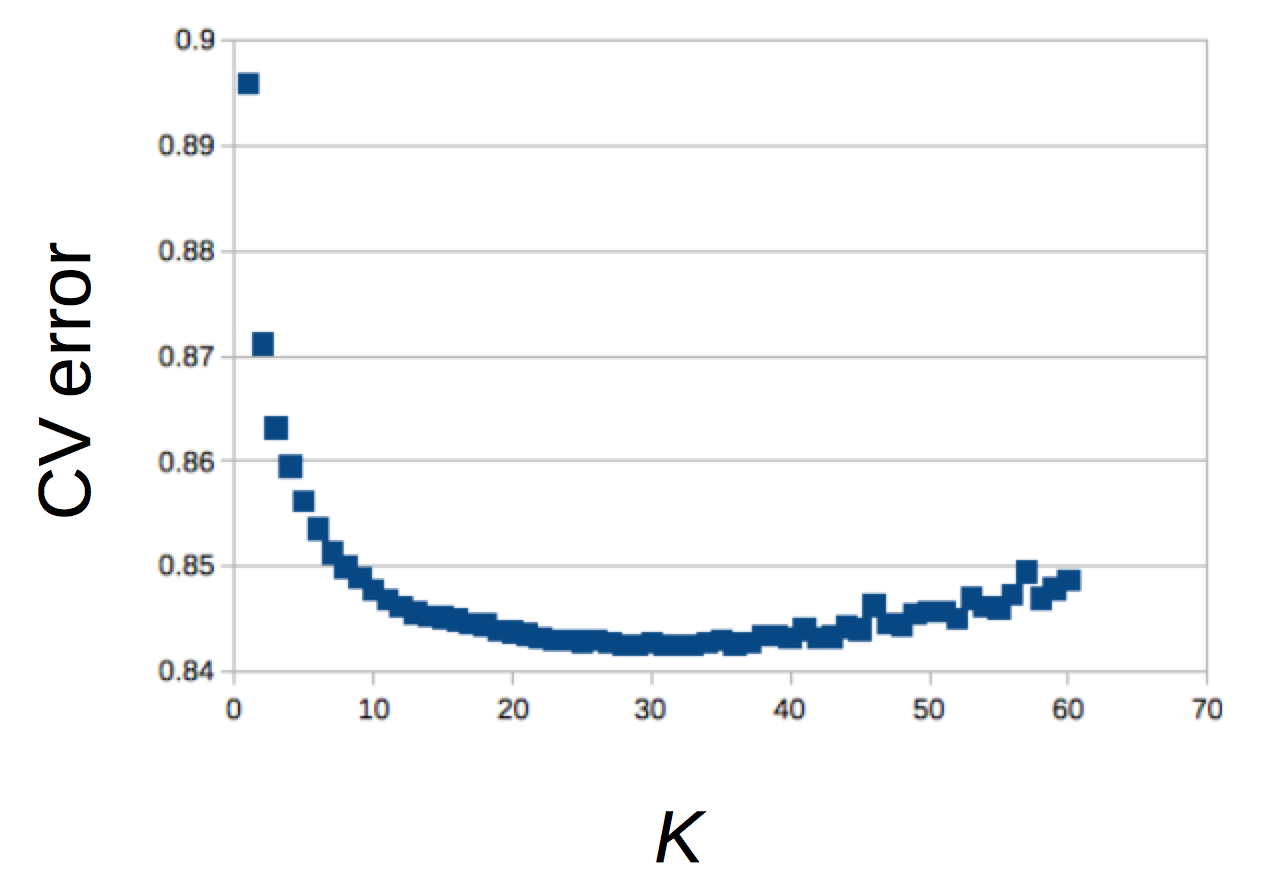
\includegraphics[width=\textwidth]{CV.png}
   \caption{\textbf{Cross validation of $\mathbf{K}$}. Optimal $K$ is found to be 28 from 1 run of ADMIXTURE 5 fold Cv on 4368 unrelated plants and and 4908 unlinked SNPs.}
  \label{figCV} 
\end{figure} 

\subsection*{Selection Scan}

I expect divergent selection in the loci involved in PSR if it is the result of local adaptation. Given the absence of opposing evolutionary forces, the main consequence of this selection is an increased frequency of adaptive alleles in populations exposed to low phosphorus availability. Therefore in order to use this pairwise difference of allele frequencies it is necessary to previously define the populations subject to comparison. From here on I will restrict the analysis to Mexican landraces and will be comparing VH(1-3) (1500 accessions) vs Mo(1-3) (507 accessions) because the Lo(1-3) landraces are a smaller set (103 accessions) and are geographically more distant from central México than Mo accessions. However the caveat that highland landraces are more frequently exposed to VH soils than lowland landraces (r = 0.39) persits so any difference in allele frequencies can be due to either environmental factor. Fst and its significance would be calculated using \texttt{hierfstat} \cite{demeeus2007}. The XP-CLR statistic will be calculated using both groups as reference \cite{chen2010}, and apropiate parameters for windows size an LD $r^2$ would be chosen as compromize between precission and computational time. The AGPv2 consensus genetic map with 7184 markers will be used as the framework for estimating the SNPs genetic distance as a required input for XP-CLR.  \url{https://ftp.maizegdb.org/MaizeGDB/FTP/B73_RefGen_v2_dumps/}.

\subsection*{Biparental Populations Analysis}

In order to clarify the role of \textit{Inv4m} in the adaptation to low soil phosphorus availability I can make use of biparental populations derived from  B73 X Palomero Toluqueño crosses. B73 is a temperate inbred that has been used as the reference genome for maize \cite{schnable2009}, while PT is a highland adapted landrace \cite{vielle-calzada2009}. Having contrasting phenotypes \ref{fig:cross} they can be used for generating segregating populations.

If \textit{Inv4m} has any role in the adaptation to low phosphorus it's introgression into a B73 genetic background could in principle improve the inbred line phosphorus starving response. Segregating introgression lines can be derived from a B73 X PT F1 through different strategies \ref{fig:hifs}. The more intuitive ones though successive back crosses, in each g{}eneration diluting the introgressing genome by half. In another method, after freezing the BC1 mosaic though several generations of selfing heterozygotes at the locus of interest are genotyped and kept so that whenever the breeder decides to autopollinate, it segregates. This method is called Heterologous Inbred Families (HIFs), each HIF having a distinct mosaic but segregating at the selected locus.

Both NIls and HIFs have segregation either 1:1 or 1:2:1. Therefore the phenotyping experiment can only be planned over the expected values of seggregation in the seed as is described in \ref{tab:table1_a}. For the HIF strategy I made a power analysis of an unbalanced ANOVA for differences in phenotypes between the three segregating clasess using custom R scripts. So for a coefficient of variation in each category phenotype of 12.5\% and a significance of 0.05 with a real difference between category means of 10\% the column n number of samples would have 90\% of power and is logistically feasible. With a cofefficient of variation of 25\% the same set samples would have just over 50\% of power.  The +P-P column lists the n appropiate for a two way ANOVA, duplicate an triplicate columns represent the amount of material needed in order to find diffrences not, beteween genotypic classes but between individual lines.


The phenotyping  experiment for phosphorus response will be set up at the LANGEBIO greenhouse at the start of the growing season (April). 3 seeds per line will be sowed into 3L pots with washed and sterilized sand with a complete randomized design. After germination only one plant per pot will be allowed to grow. The substrate will be watered every 3 days with 200 mL of +P (\SI{330}{\micro\molar}) or -P (\SI{0}{\micro\molar}) modified Hoagland solution \cite{salazar-vidal2016, hoagland1936}.  At 25 days after emergence  measurements of shoot length, number of leaves, root length root/shoot ratio will be taken and tissue for genotyping and metabolomics will be sampled, flash frozen, and preserved at -80oC. Phosphorus Ionomics will be carried out with ICP-MS by Ivan Baxter, in the Missouri Danforth center.



\begin{figure}[!h]
   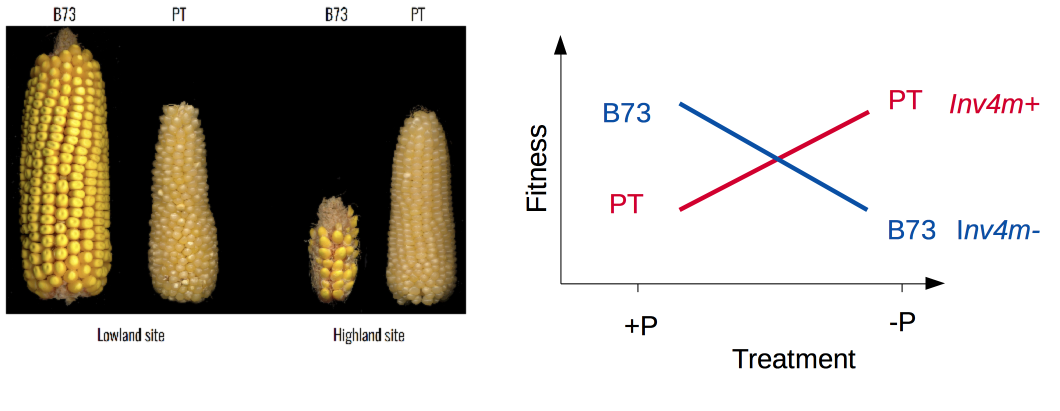
\includegraphics[width=\textwidth]{cross.png}
   \caption{\textbf{Contrasting phenotypes of B73 and PT}. Left: Actual phenotype of B73 aand PT in high and low altitude (photo Rubén Rellán). Right: Expected reaction curves of B73 and PT if \textit{Inv4m} plays a  crucial in localad aptation to low phosphorus availability through a genetic trade-off. 
  \label{fig:cross} }
\end{figure} 

\begin{figure}[!h]
   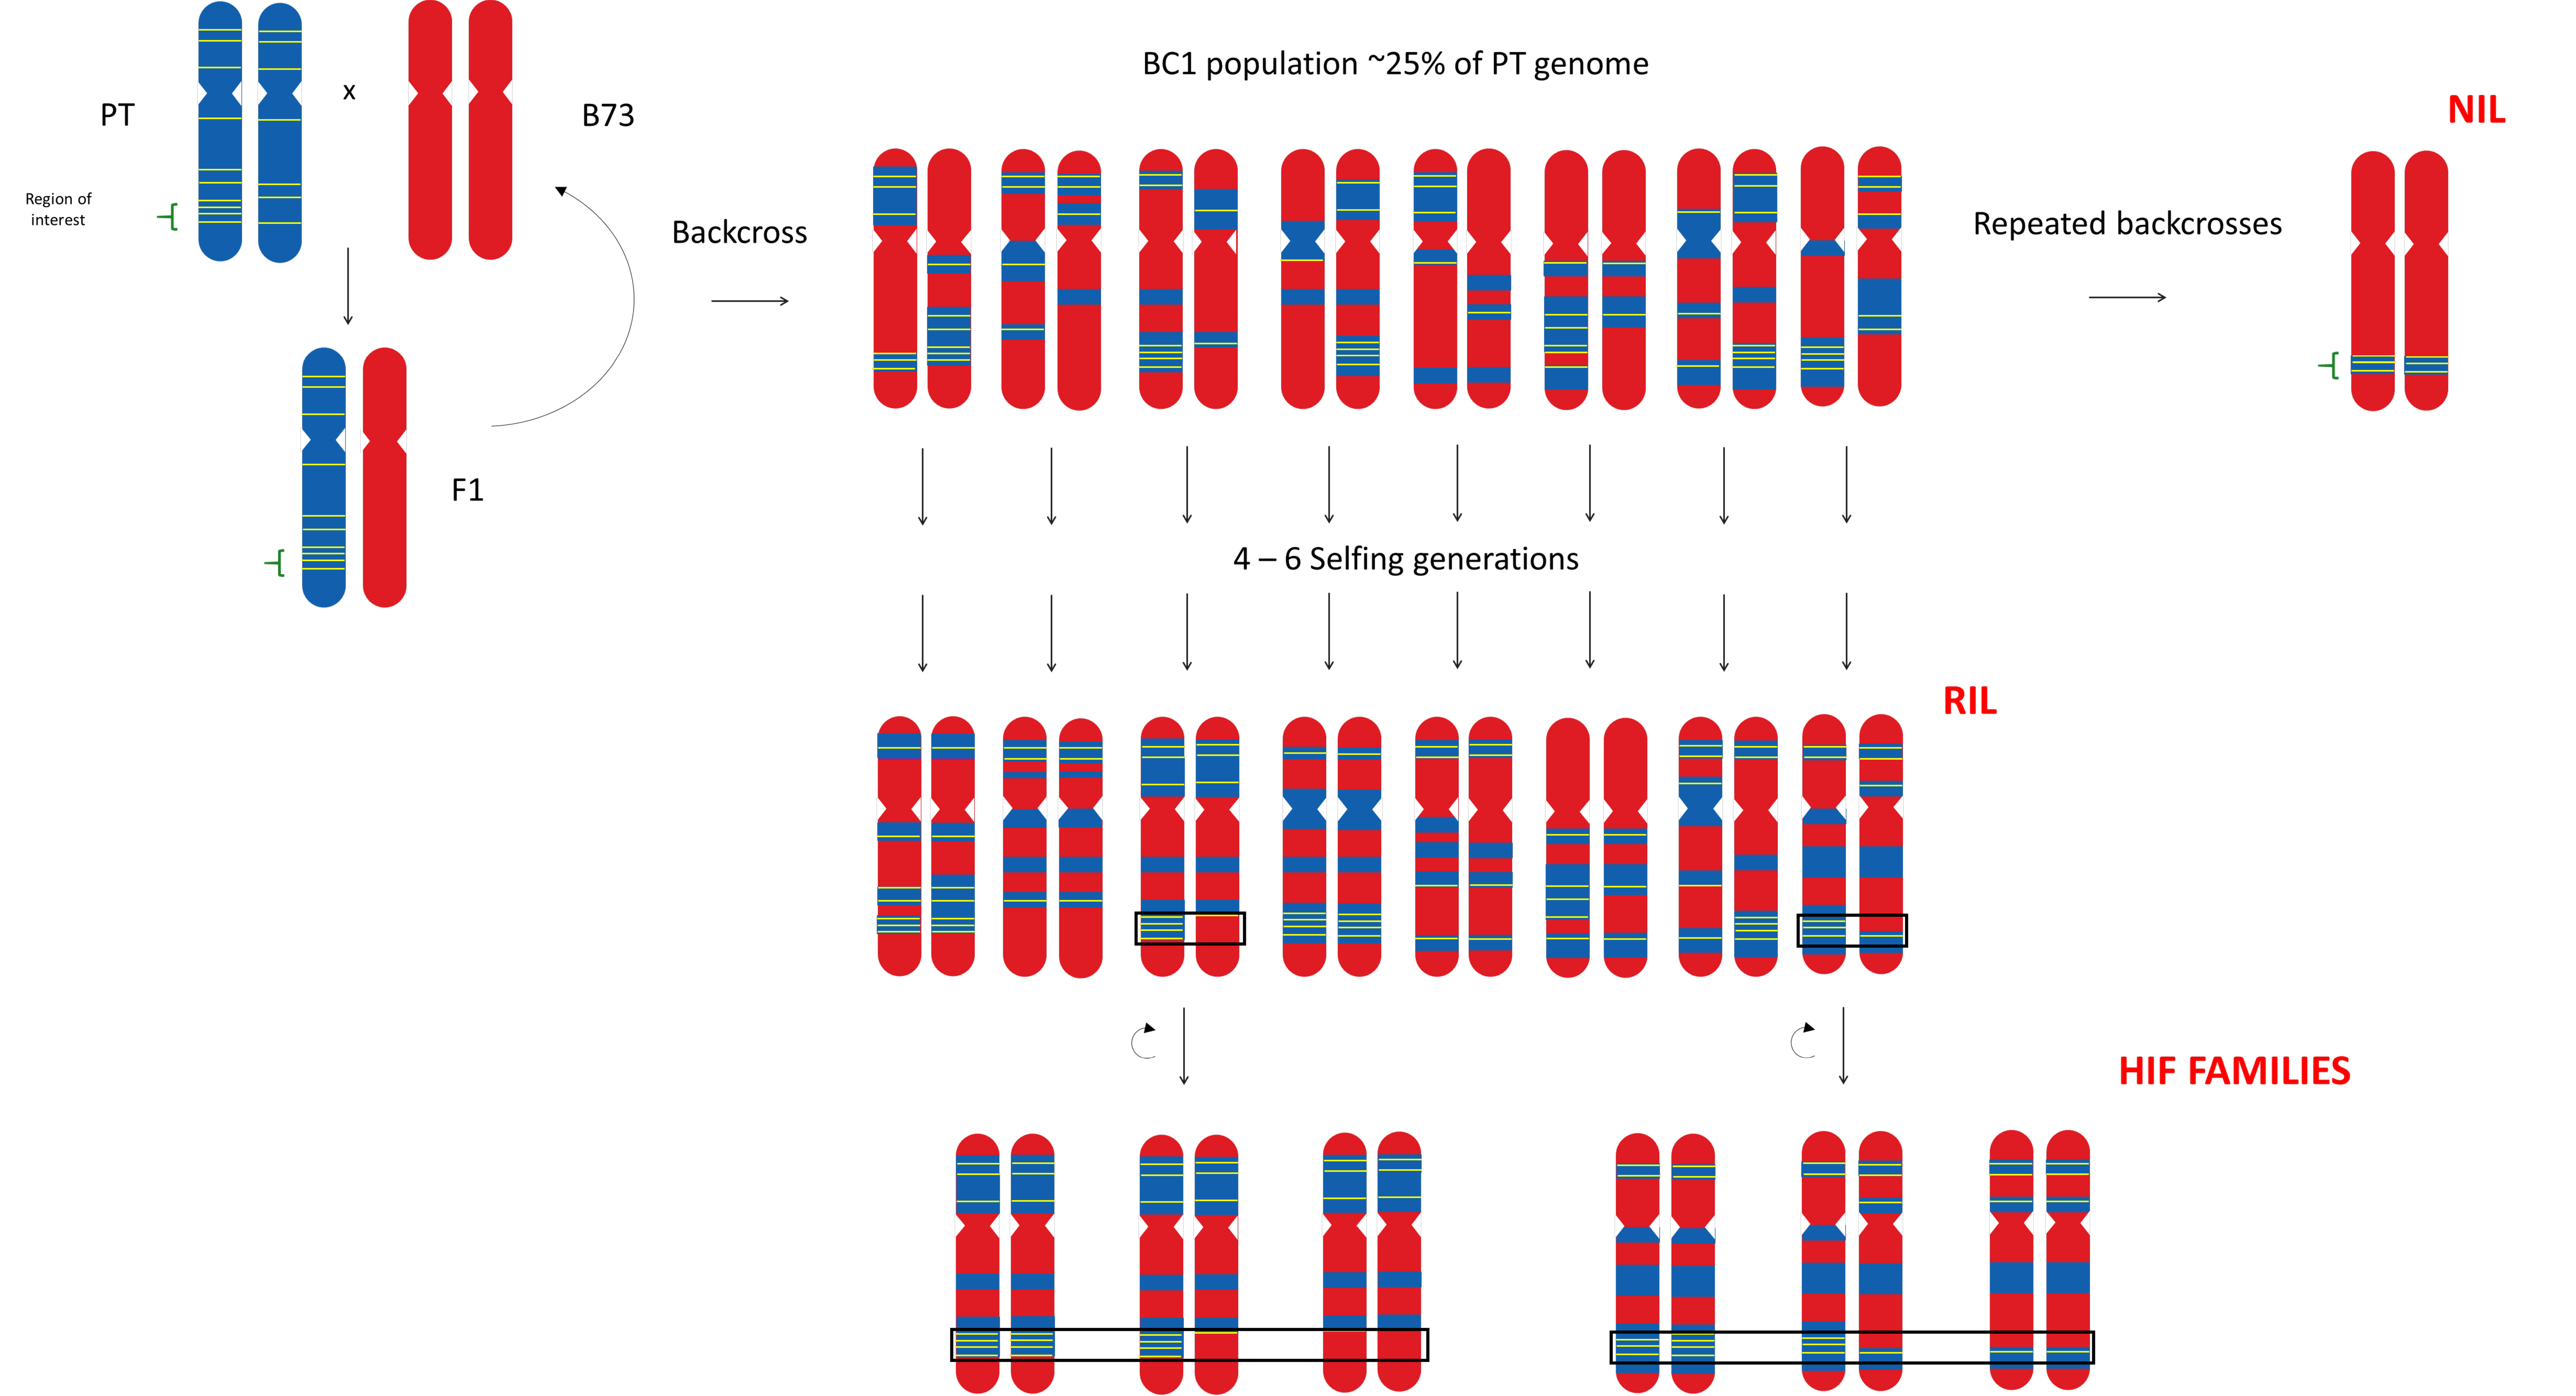
\includegraphics[width=\textwidth]{hifs.pdf}
   \caption{\textbf{Crossing scheme for genetic analysisof B73 and PT}.Reproduced from \cite{aguilarrangel2018}}
  \label{fig:hifs} 
\end{figure} 


% Please add the following required packages to your document preamble:
% {}
\begin{table}[!h]
\caption {\label{tab:cap} \textbf{CAPS marker at the \textit{inv4m}, modified from  \cite{aguilarrangel2018}}}
\begin{center}
\begin{adjustbox}{width=0.9\textwidth}
\begin{tabular}{@{}lll@{}}
\toprule
\textbf{Properties} &                                                    &  \\ \midrule
Oligo code               & RS 427/428                                         &  \\
SNP id                & PZE104103103                                       &  \\
Position (bp)            & 179617762                                          &  \\
Primer forward           & \texttt{CTGAGCAGGAGATGATGGCCACTC } &  \\
Primer reverse           & \texttt{GGAAAGGACATAAAAGAAAGGTGCA} &  \\
5' context (50 bp) & \texttt{aagaagatgcatgaatggttttgcacgtagcacttgctagggcgtacgca} &  \\
B73 allele (ref)         & \texttt{A}                                                  &  \\
PT allele (alt)          & \texttt{G}                                                  &  \\
3' context (30 bp) & \texttt{attcttcttcttggcccttgtgaattccgaattctcgacgattgattctg} &  \\
Amplicon size (bp)       & 502                                                &  \\
Restriction Enzyme       & \textit{Hinf} I                                             &  \\
B73 fragments  (bp)      & 166; 44; 251; 61                                   &  \\
PT fragments    (bp)     & 166; 295; 61                                       &  \\ \bottomrule
\end{tabular}
\end{adjustbox}
\end{center}
\end{table}


\begin{table}[!h]
\caption{\textbf{Plant material requirements for HIF design.}}


\begin{subtable}{\textwidth}
\centering
\begin{tabular}{lrrrr}
                  & \multicolumn{1}{l}{}           & \multicolumn{1}{l}{}               & \multicolumn{1}{l}{}                   & \multicolumn{1}{l}{}                     \\
\textbf{genotype} & \multicolumn{1}{l}{\textbf{n}} & \multicolumn{1}{l}{\textbf{+P/-P}} & \multicolumn{1}{l}{\textbf{Duplicate}} & \multicolumn{1}{l}{\textbf{Triplicate}}  \\ 
\hline
inv+      & 25                       & 50                        & 100                           & 150                             \\
inv+/inv- & 50                       & 100                       & 200                           & 300                             \\
inv-      & 25                       & 50                        & 100                           & 200                             \\
B73       & 20                       & 40                        & 80                            & 160                             \\
PT        & 20                       & 40                        & 80                            & 160 \\
\cline{2-5}
          & \multicolumn{1}{l}{pots} & 280                       & 560                           & 650                             \\
          & \multicolumn{1}{l}{seed} & 840                       & 1680                          & 1950                                       
\end{tabular}
\caption{ \textbf{HIF Lines}}
\label{tab:table1_a}
\end{subtable}

\begin{subtable}{\textwidth}
\centering
\begin{tabular}{lrrrr}
                  & \multicolumn{1}{l}{}           & \multicolumn{1}{l}{}               & \multicolumn{1}{l}{}                   & \multicolumn{1}{l}{}                     \\
\textbf{genotype} & \multicolumn{1}{l}{\textbf{n}} & \multicolumn{1}{l}{\textbf{+P/-P}} & \multicolumn{1}{l}{\textbf{Duplicate}} & \multicolumn{1}{l}{\textbf{Triplicate}}  \\ 
\hline
inv+/inv- & 25                       & 50                        & 100                           & 150                             \\
inv-      & 20                       & 40                        & 80                            & 120                             \\
B73       & 10                       & 20                        & 40                            & 60                              \\
PT        & 10                       & 20                        & 40                            & 60                              \\
                                      \\ 
\cline{2-5}
          & \multicolumn{1}{l}{pots} & 280                       & 260                           & 270                             \\
          & \multicolumn{1}{l}{seed} & 840                       & 780                           & 810                                      
\end{tabular}
\caption{ \textbf{NIL Lines}}
\label{tab:table1_b}
\end{subtable}
\end{table}

% newpage forces a page break if you want to clearly separate materials from results
\clearpage

\section*{Environmental GWAS Results}
\begin{figure}[!b] %s state preferences regarding figure placement here
\centering
\begin{subfigure}[h]{0.4\linewidth}
   \centering
   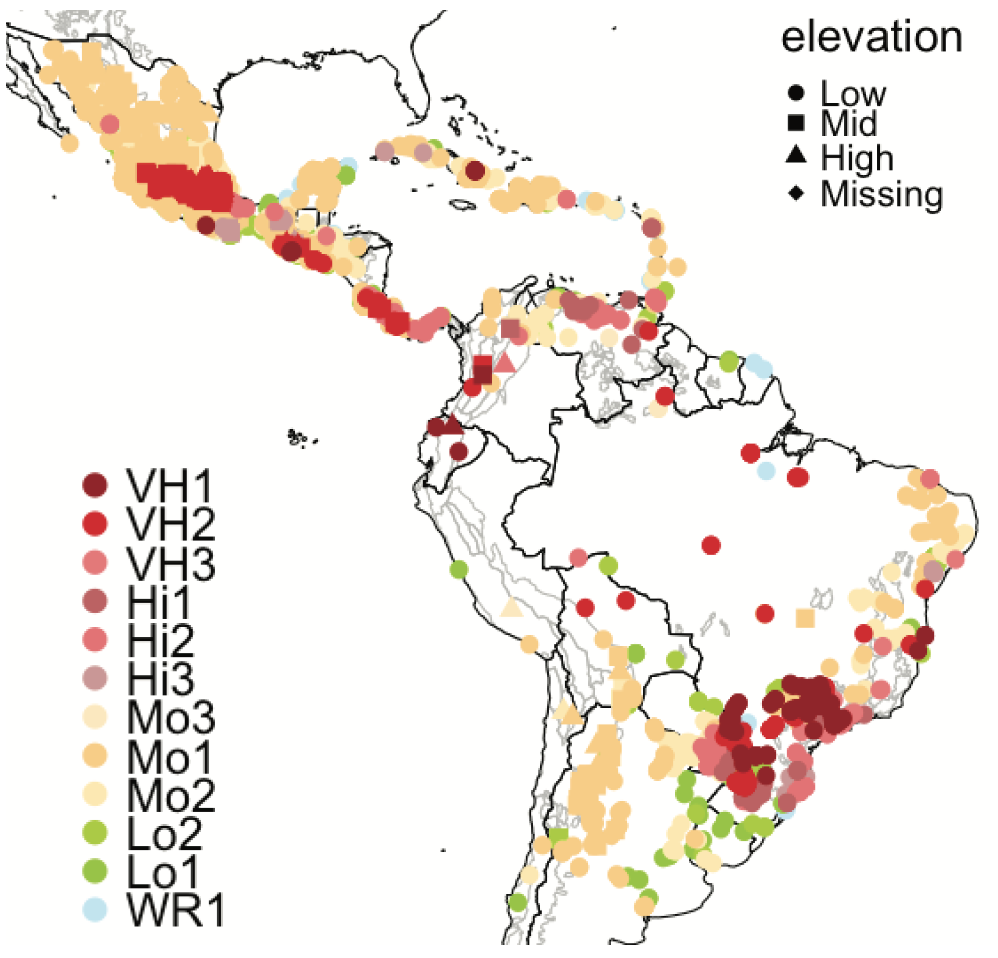
\includegraphics[width=\linewidth]{fig3a.png}
   \caption{}
   \label{fig:fig3a}
\end{subfigure}
\hfill
\begin{subfigure}{0.4\linewidth}
   \centering
   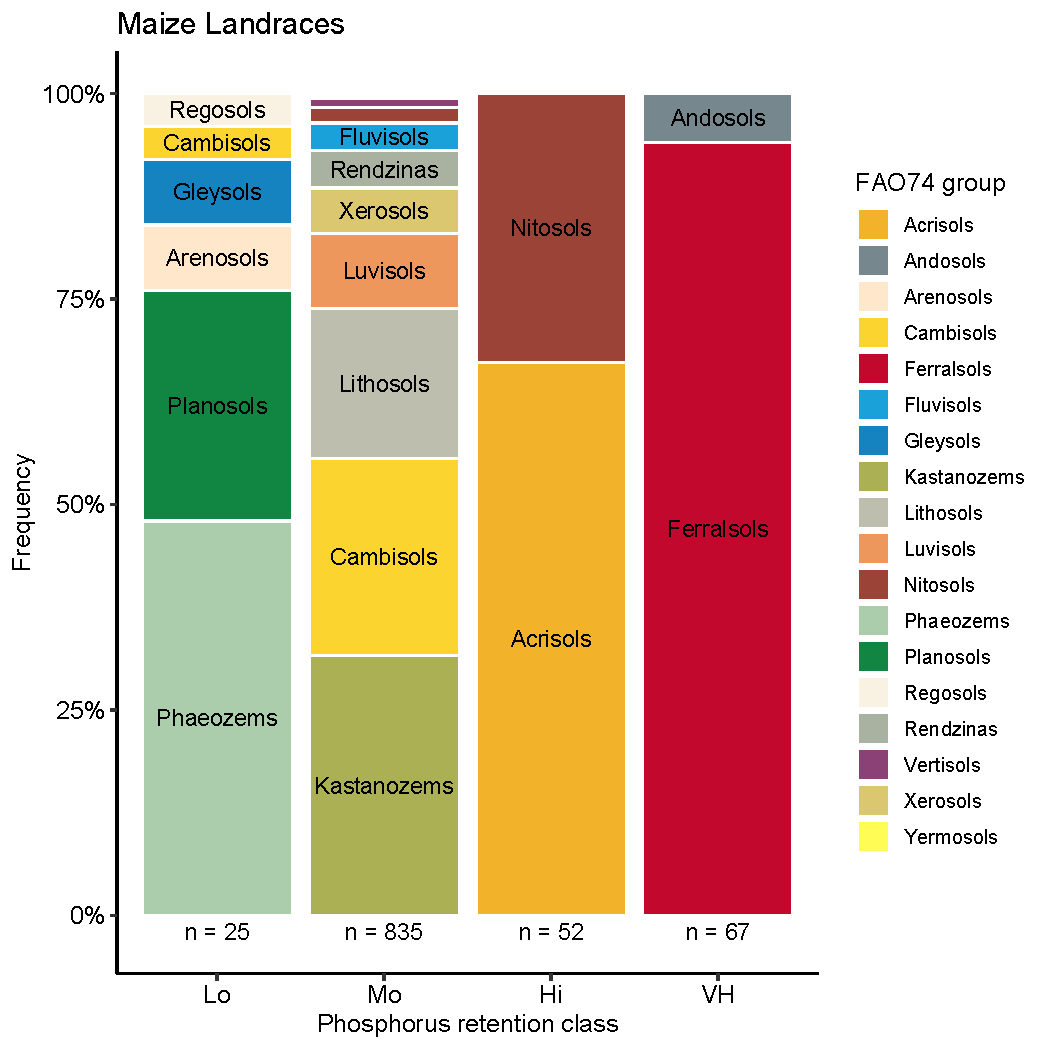
\includegraphics[width=\linewidth]{fig3.pdf}
   \caption{}
   \label{fig:fig3c}
\end{subfigure}
\\[\baselineskip]
   \begin{subfigure}{0.5\linewidth}
   \centering
   \includegraphics[width=\linewidth]{fig3c.png}
   \caption{}
   \label{fig:fig3b} 
\end{subfigure}

\centering

\caption{\textbf{Phosphorus retention potential for LAC landraces, soil distribution and correlation with selected confounding variables}. \textbf{(a)}Distribution map of 3238 geolocated landraces from \cite{romeronavarro2017},  most of landraces were collected form sites with moderate phosphorus retention potential. There is a lack of sampling in the Northern and Central Andes. \textbf{(b)} Soil distribution among phosphorus retention potential classes. The counted landraces (n) are those that happen to be in locations with 100\% probability for their phosphorus retention class. VH soils are restricted to andosols and ferralsols. Hi soils are limited to acrisoils and nitosols. The moderate class is the most abundant and most eclectic, but dominated by kastanozems, cambisols and lithosols. The Lo class is dominated by phaeozems and planosols. \textbf{(c)} Altitude correlates moderately with VH and Hi retention potential which can be due to a higher proportion of andosols in the Mexican transvolcanic belt, and a higher  proportion of acrisols in southern Brazil and Venezuelan northeast lowlands. Non significant correlations are marked with a cross (t test, Bonferroni corrected $p < 0.05/36$).}

\label{fig3} % \label works only AFTER \caption within figure environment

\end{figure}


\begin{figure}[p] %s state preferences regarding figure placement here

% use to correct figure counter if necessary
%\renewcommand{\thefigure}{2}
\centering

\begin{subfigure}[b]{\textwidth}
   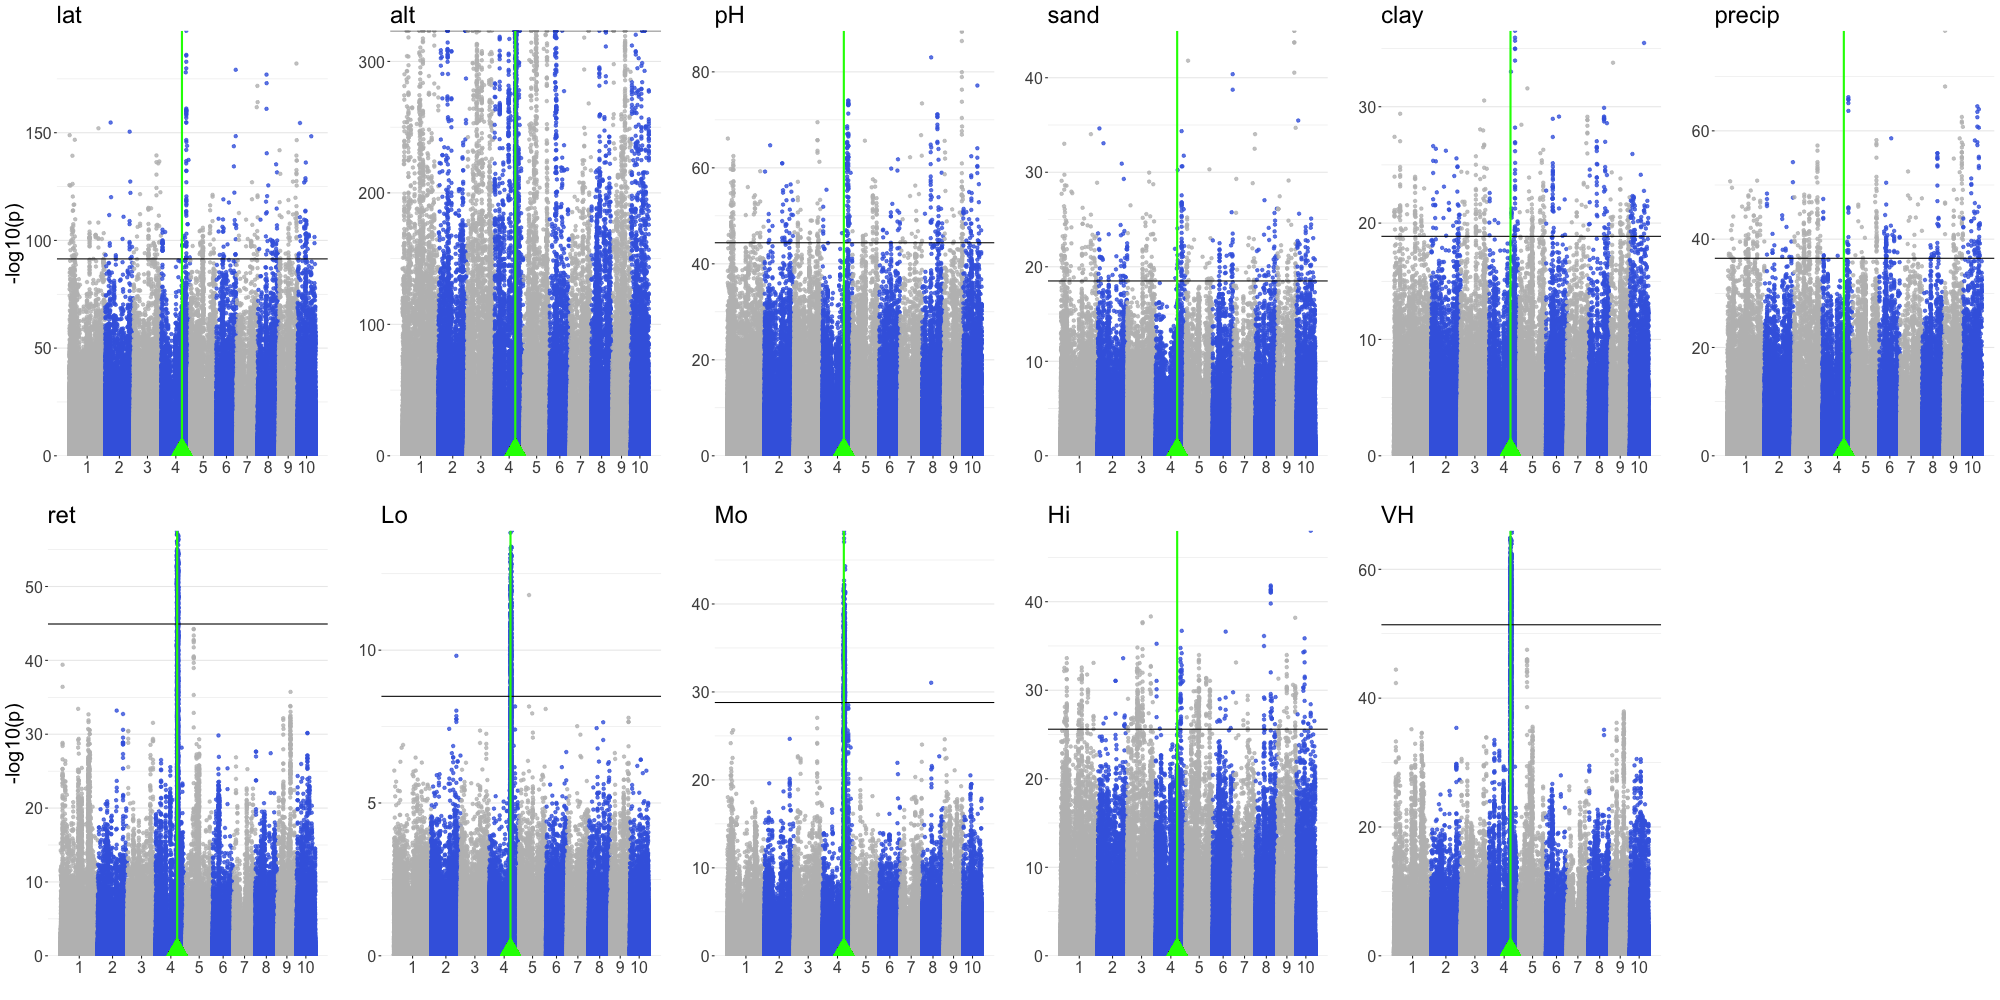
\includegraphics[width=\linewidth]{fig4.png}
   \label{fig:fig4top} 
   \caption{\textbf{Genomewide}. For the phosphorus retention variables (bottom panel) the strongest association is observed in Chromosome 4 near 172 Mb (green triangle). A GWAS peak is detected in the same location for altitude (alt, top panel).} 

   \bigskip

\end{subfigure} 

\begin{subfigure}[b]{\textwidth}
   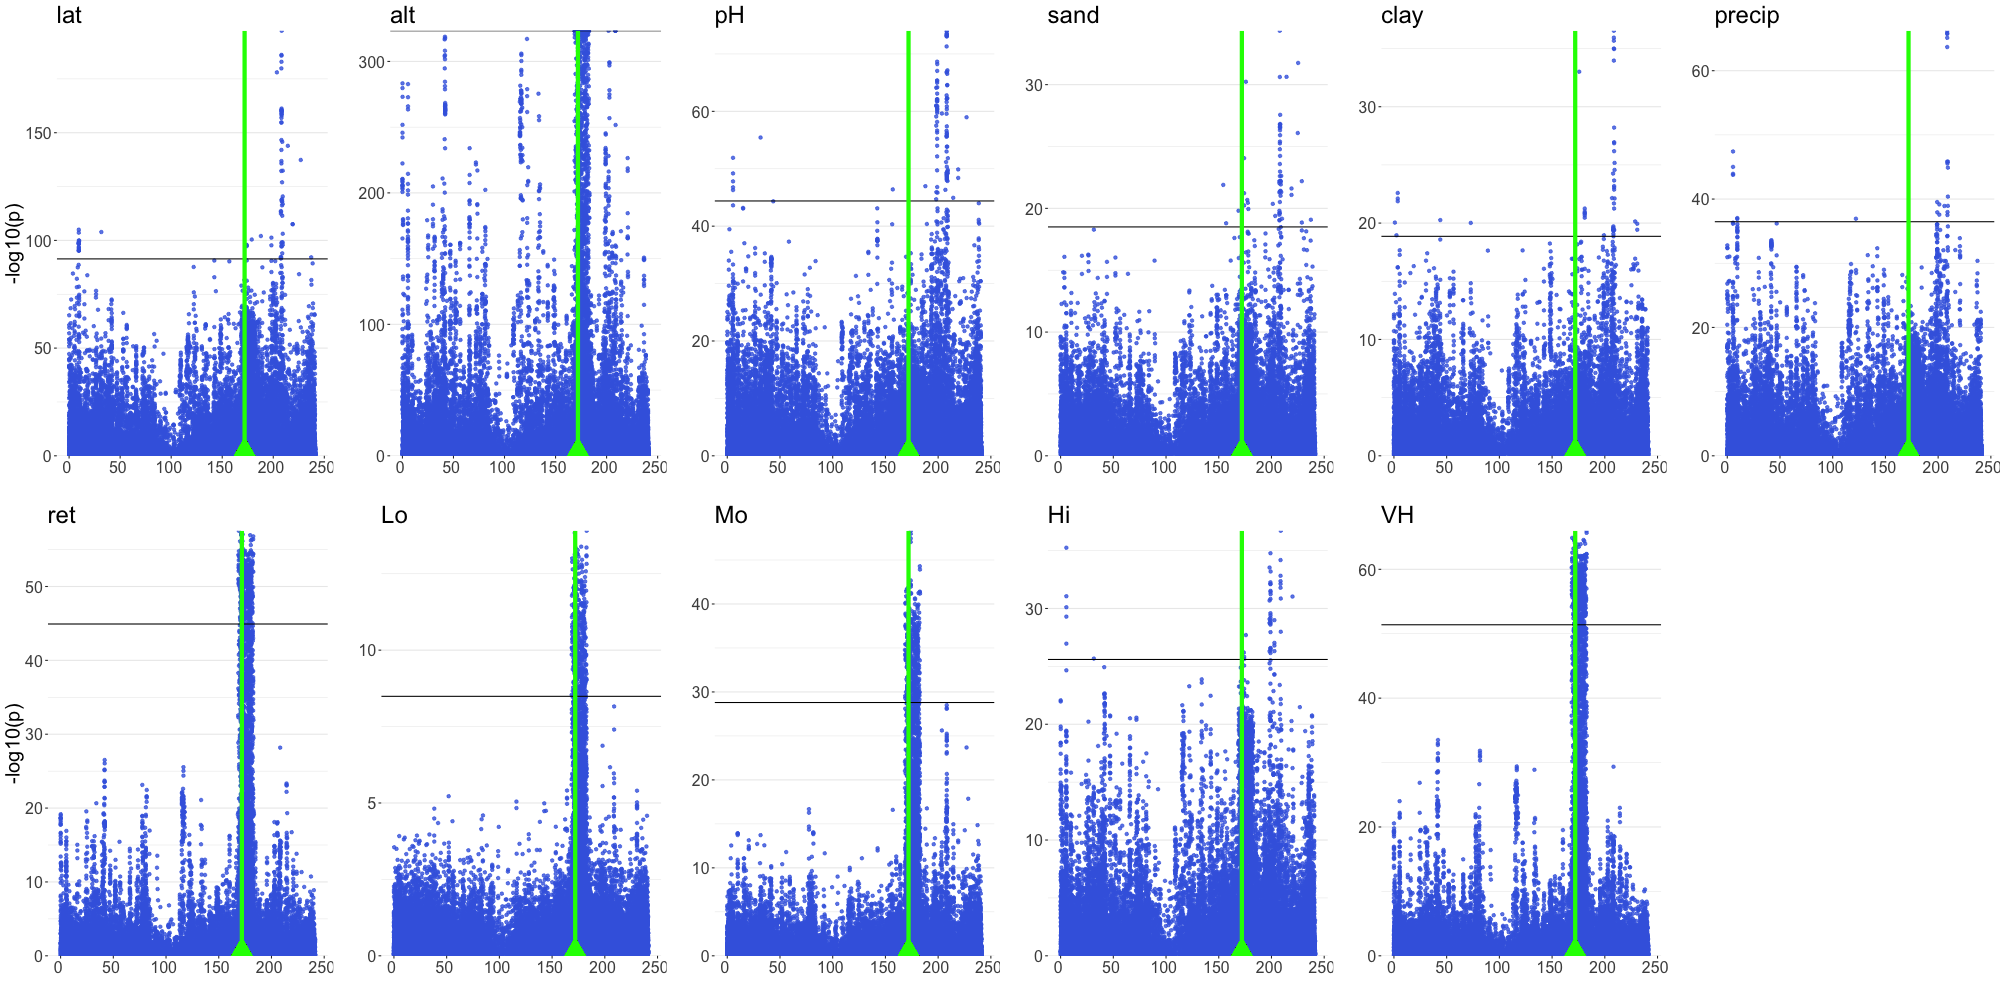
\includegraphics[width=\linewidth]{fig5.png}
   \label{fig:fig5top} 
   \caption{\textbf{Chromosome 4}. A zoom into this chromosome shows that the signal around 172 Mb is characteristic of altitude and the phosphorus retention variables except Hi. Despite the significant correlations observed in Figure \ref{fig3}, latitude, precipitation, and the other 3 soil variables do not show as strong association in this region.}
   \bigskip

\end{subfigure} 

\caption{\textbf{GLM GWAS analysis.} Black horizontal bar corresponds to  0.001 quantile of p-values.}
\label{fig5}

\end{figure}

\begin{figure}[p] %s state preferences regarding figure placement here

% use to correct figure counter if necessary
%\renewcommand{\thefigure}{2}
\centering

\begin{subfigure}[b]{\textwidth}
   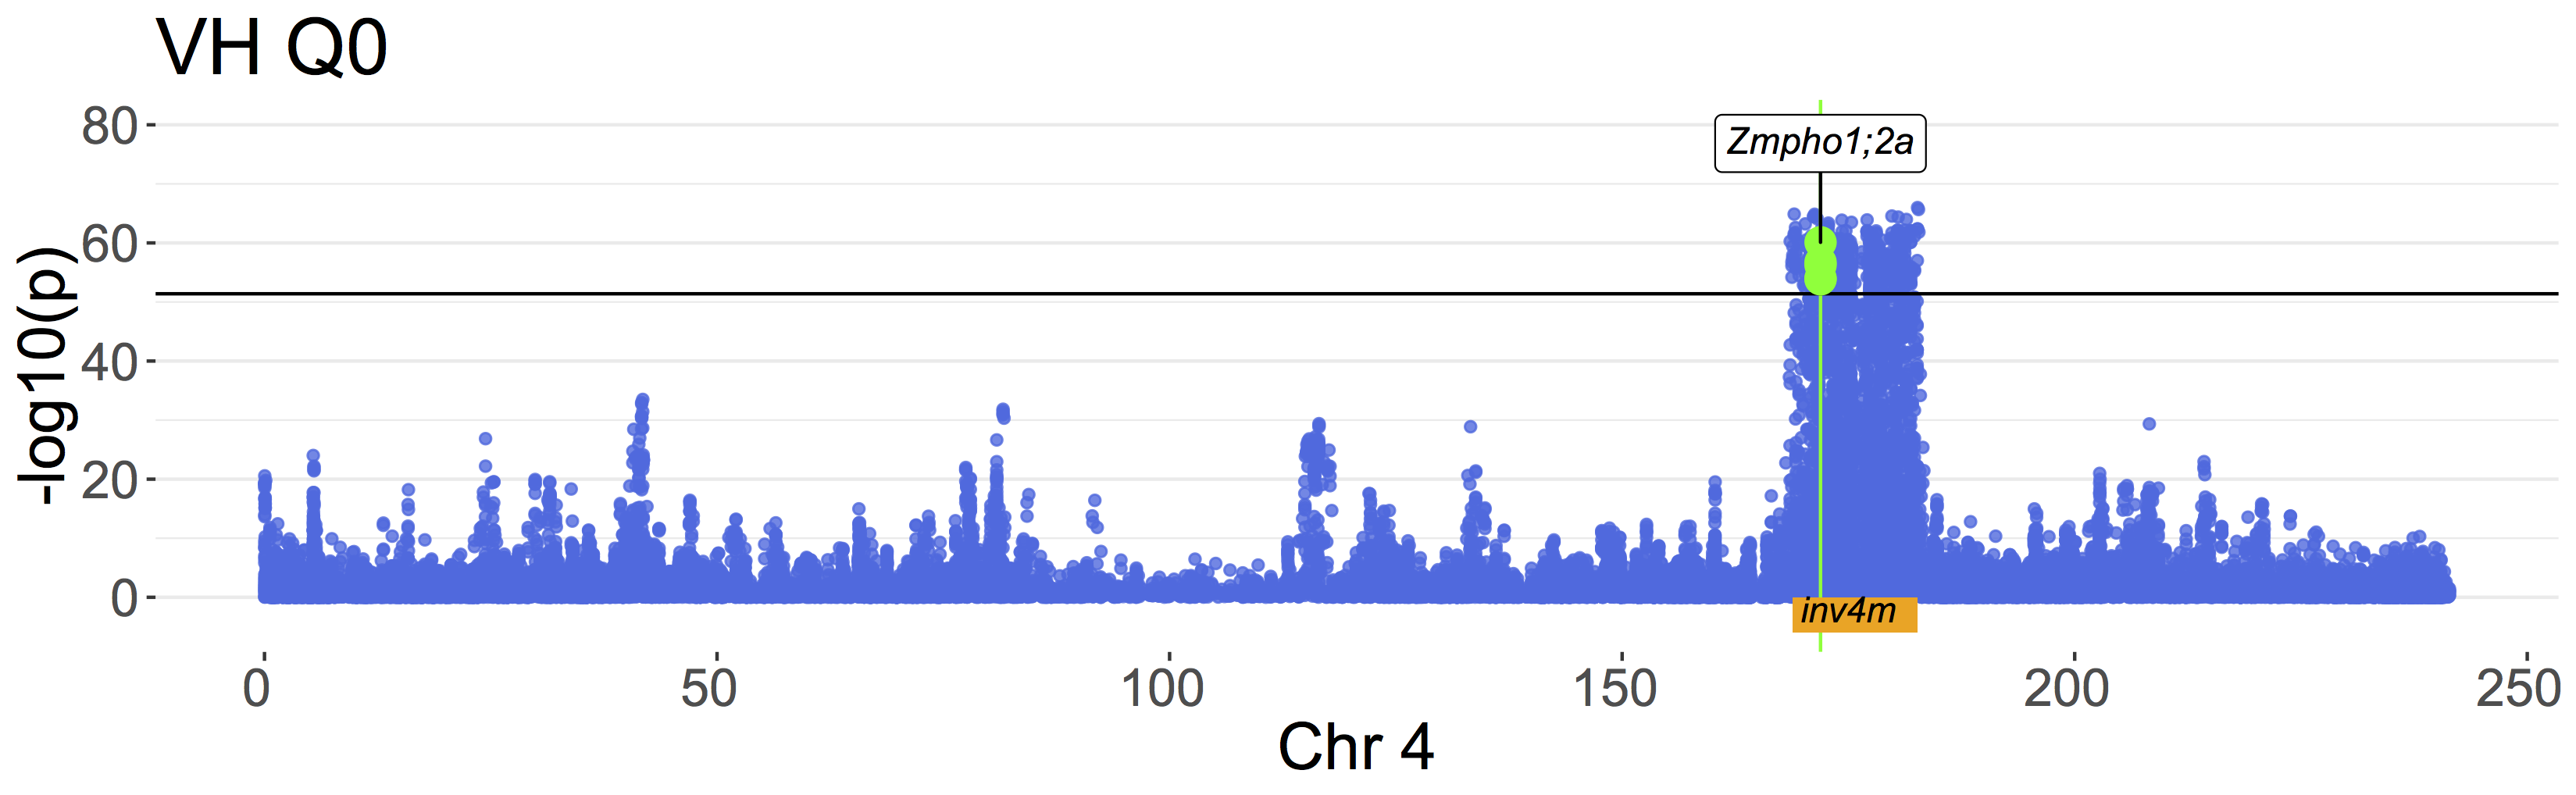
\includegraphics[width=\linewidth]{fig6a.png}
   \caption{}
\end{subfigure} 

\begin{subfigure}[b]{\textwidth}
   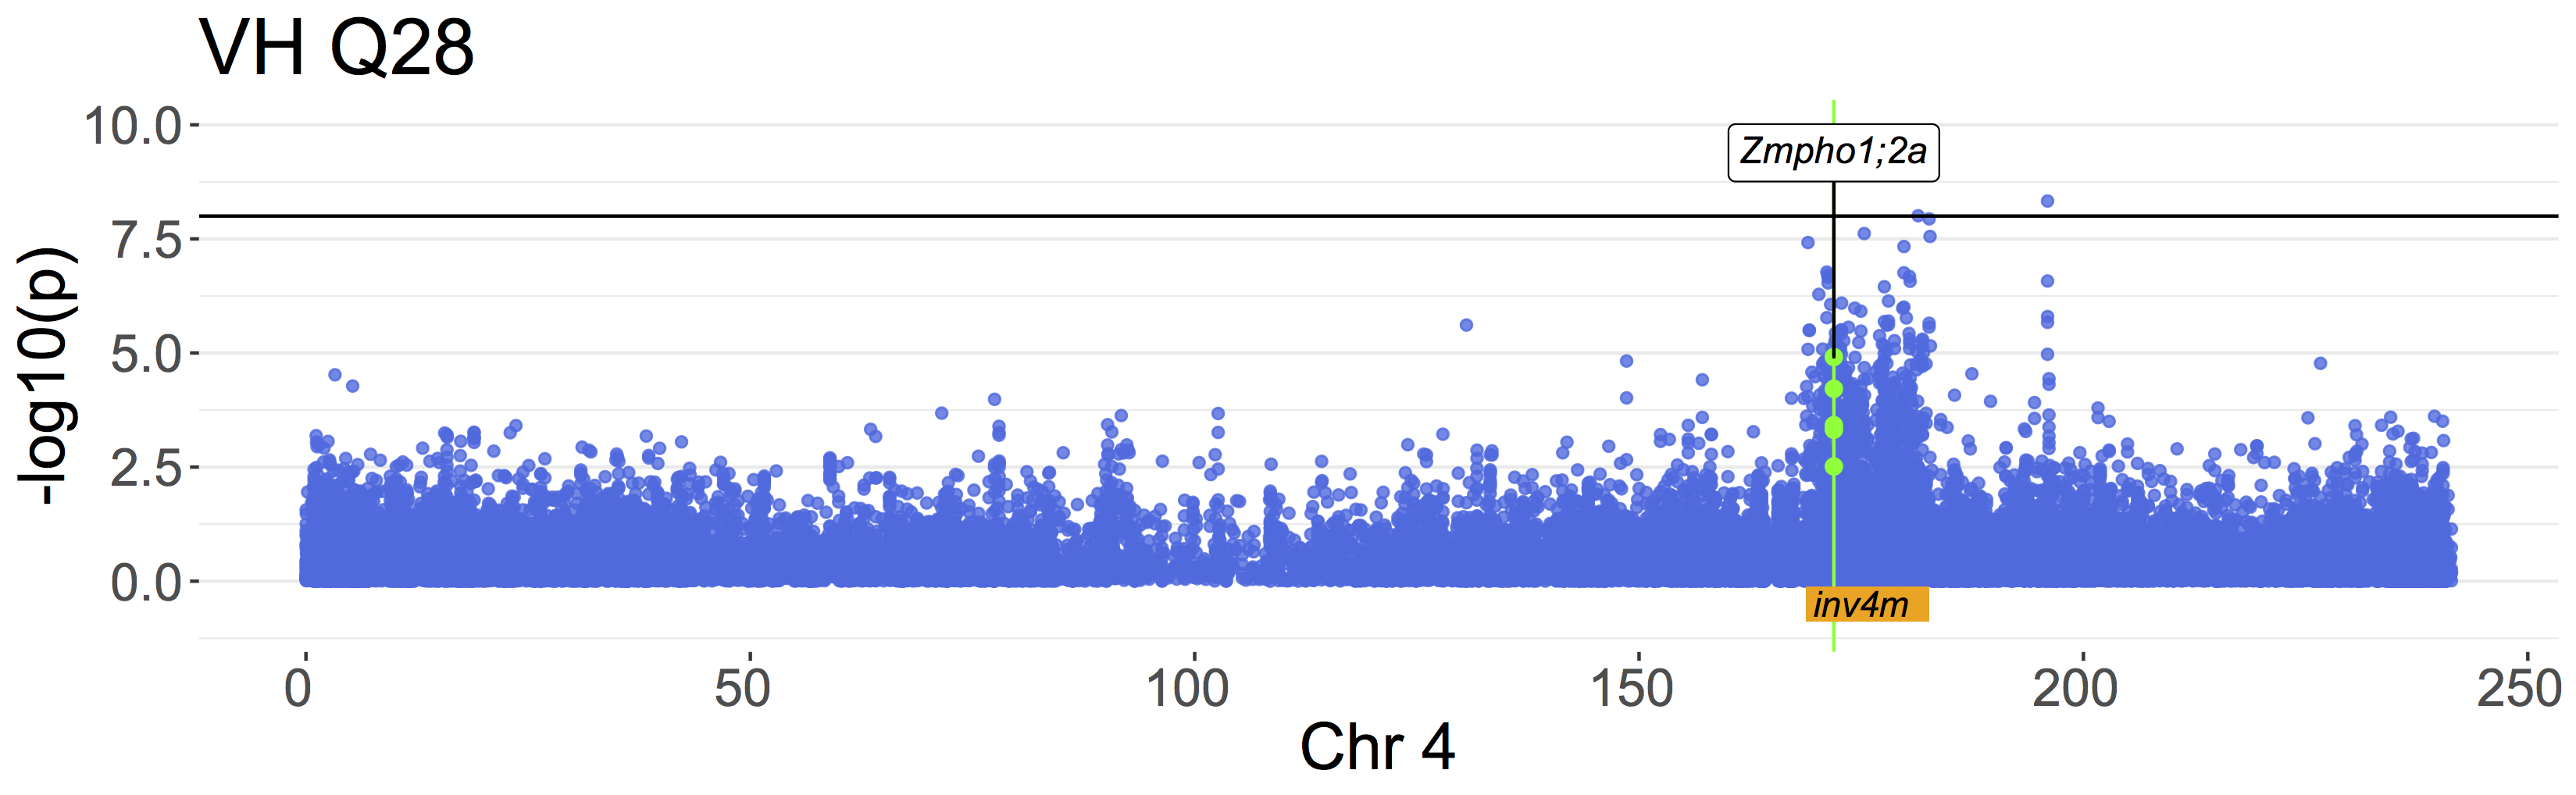
\includegraphics[width=\linewidth]{fig6b.png}
    \caption{}
\end{subfigure} 
\\[\baselineskip]
\begin{subfigure}[t]{0.45\textwidth}
   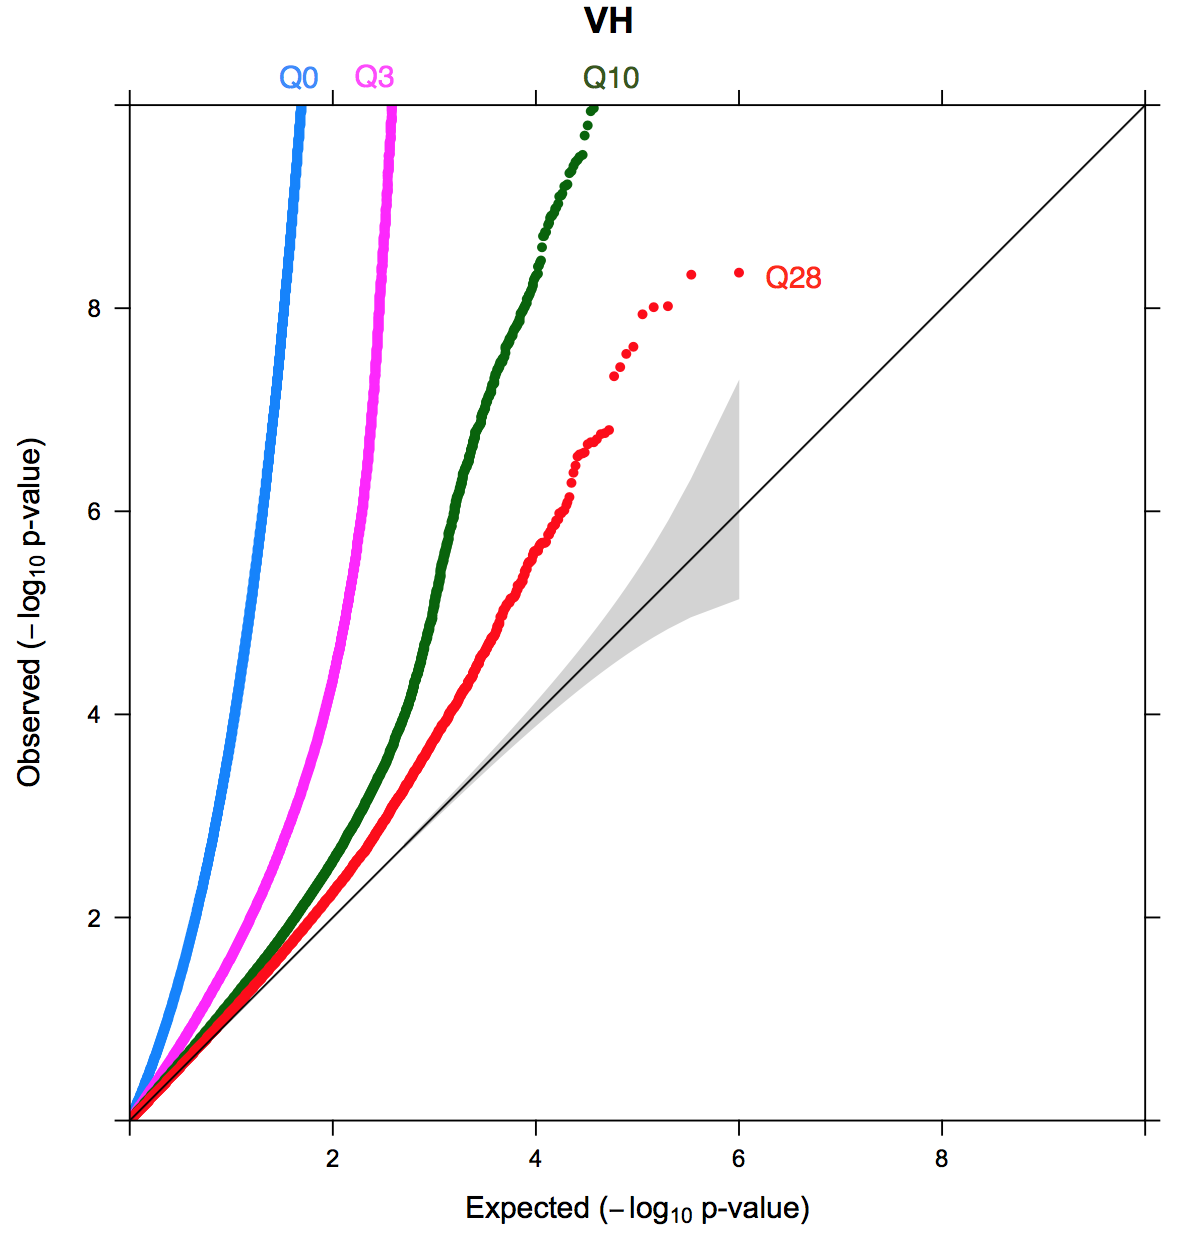
\includegraphics[width=\linewidth]{fig6c.png}  
    \caption{}    
\end{subfigure}
\hfill
\begin{subfigure}[t]{0.45\textwidth}
   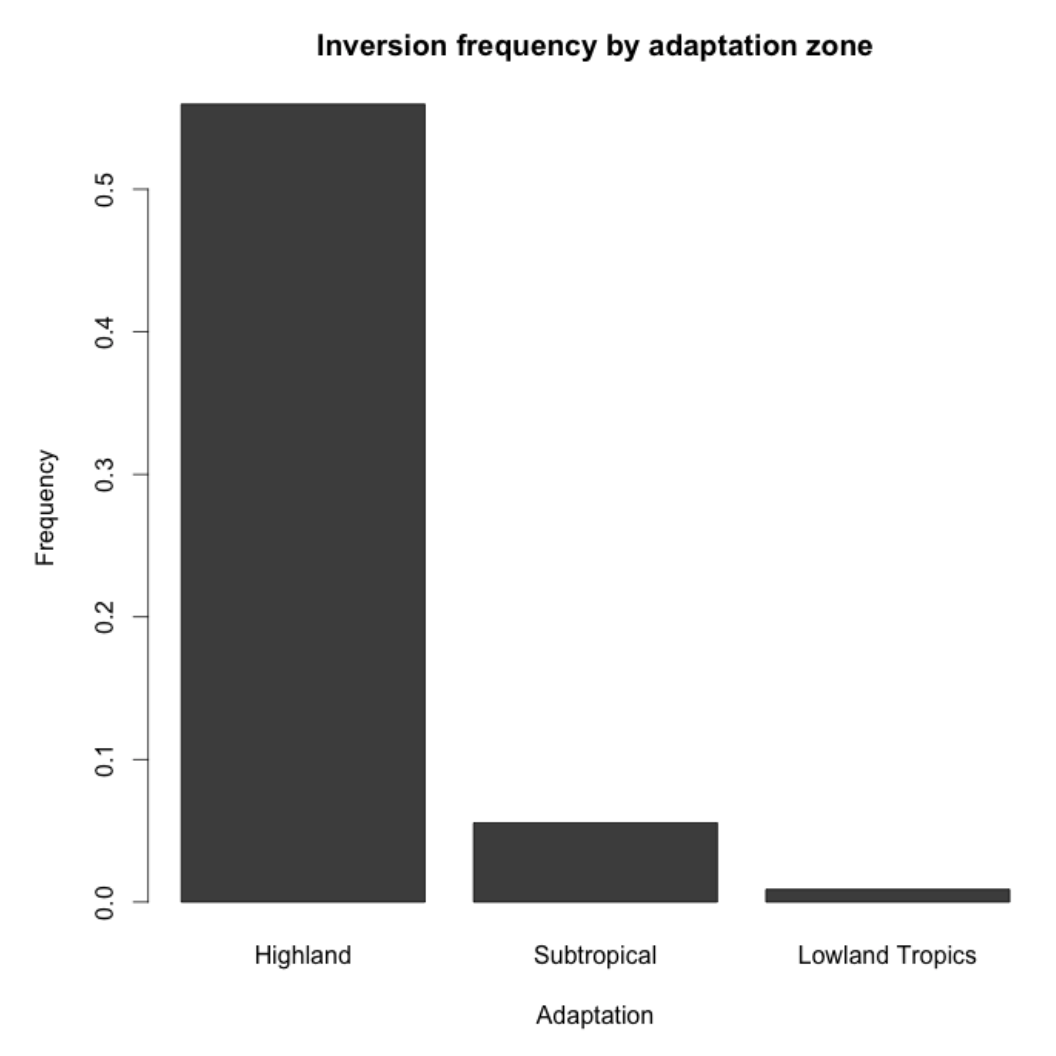
\includegraphics[width=\linewidth]{fig6d.png}
    \caption{}
       \bigskip
\end{subfigure}
\caption{\textbf{GWAS main signal is lost with population structure correction and corresponds to \textit{Inv4m}, an inversion mostly present in highland landraces.} VH is used as phenotype for ilustration. Population structure was accounted for with Q,  the ancestry coefficient matrix of \textit{K} subpopulations (\textit{K} = 0, 3, 10, 28 estimated with \cite{alexander2009}), included as fixed effect in the GWAS GLM model. \textit{Inv4m} is a putative adaptive introgression from highland teosinte spanning 13 Mb, (orange bar) \cite{pyhajarvi2013},  \textbf{(a)} At Q0, no ancestry matrix included, there are 4  significant snps (green dots) in the phosphate transporter \textit{ZmPho1;2a} \cite{salazar-vidal2016} (green line at 172 Mb),  black line 0.001 p-value quantile. \textbf{(b)} Most of the significance is lost at Q28,  black line p-value = 1e-8. \textbf{(c)} GWAS QQ-plot, p-values are far more significant than expected (over the diagonal) for any Q. Increasing the number of postulated subpopulations diminishes p-value inflation but even at Q28 they deviate from the 95\% CI (grey). \textbf{(d)}  \textit{Inv4m} is mostly present in highland landraces (2000 m.a.s.l)\cite{romeronavarro2017}.}

\label{fig6}

\end{figure}


% \begin{figure}[p] %s state preferences regarding figure placement here

% % use to correct figure counter if necessary
% %\renewcommand{\thefigure}{2}

% 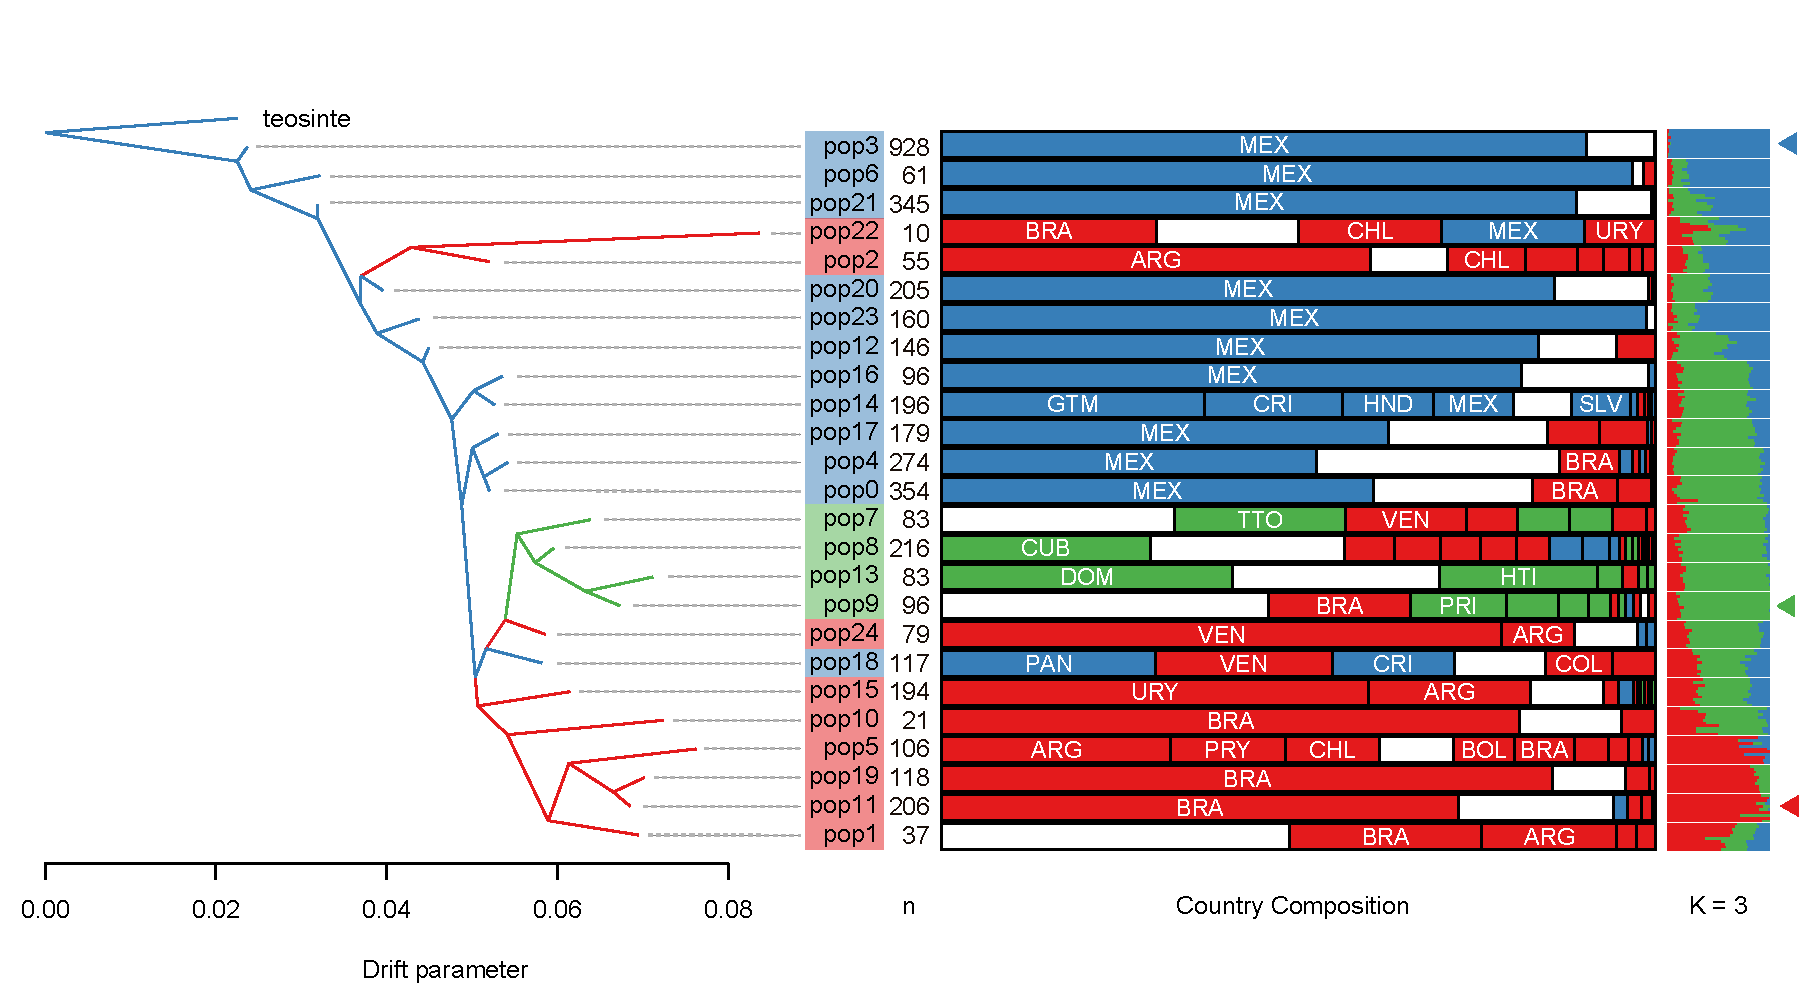
\includegraphics[width=\textwidth]{fig7.pdf}

% \caption{\color{Gray} \textbf{Demographic history K = 25}.}

% \label{fig7} % \label works only AFTER \caption within figure environment

% % \end{figure}

% % \begin{figure}[p] %s state preferences regarding figure placement here

% % use to correct figure counter if necessary
% %\renewcommand{\thefigure}{2}

% 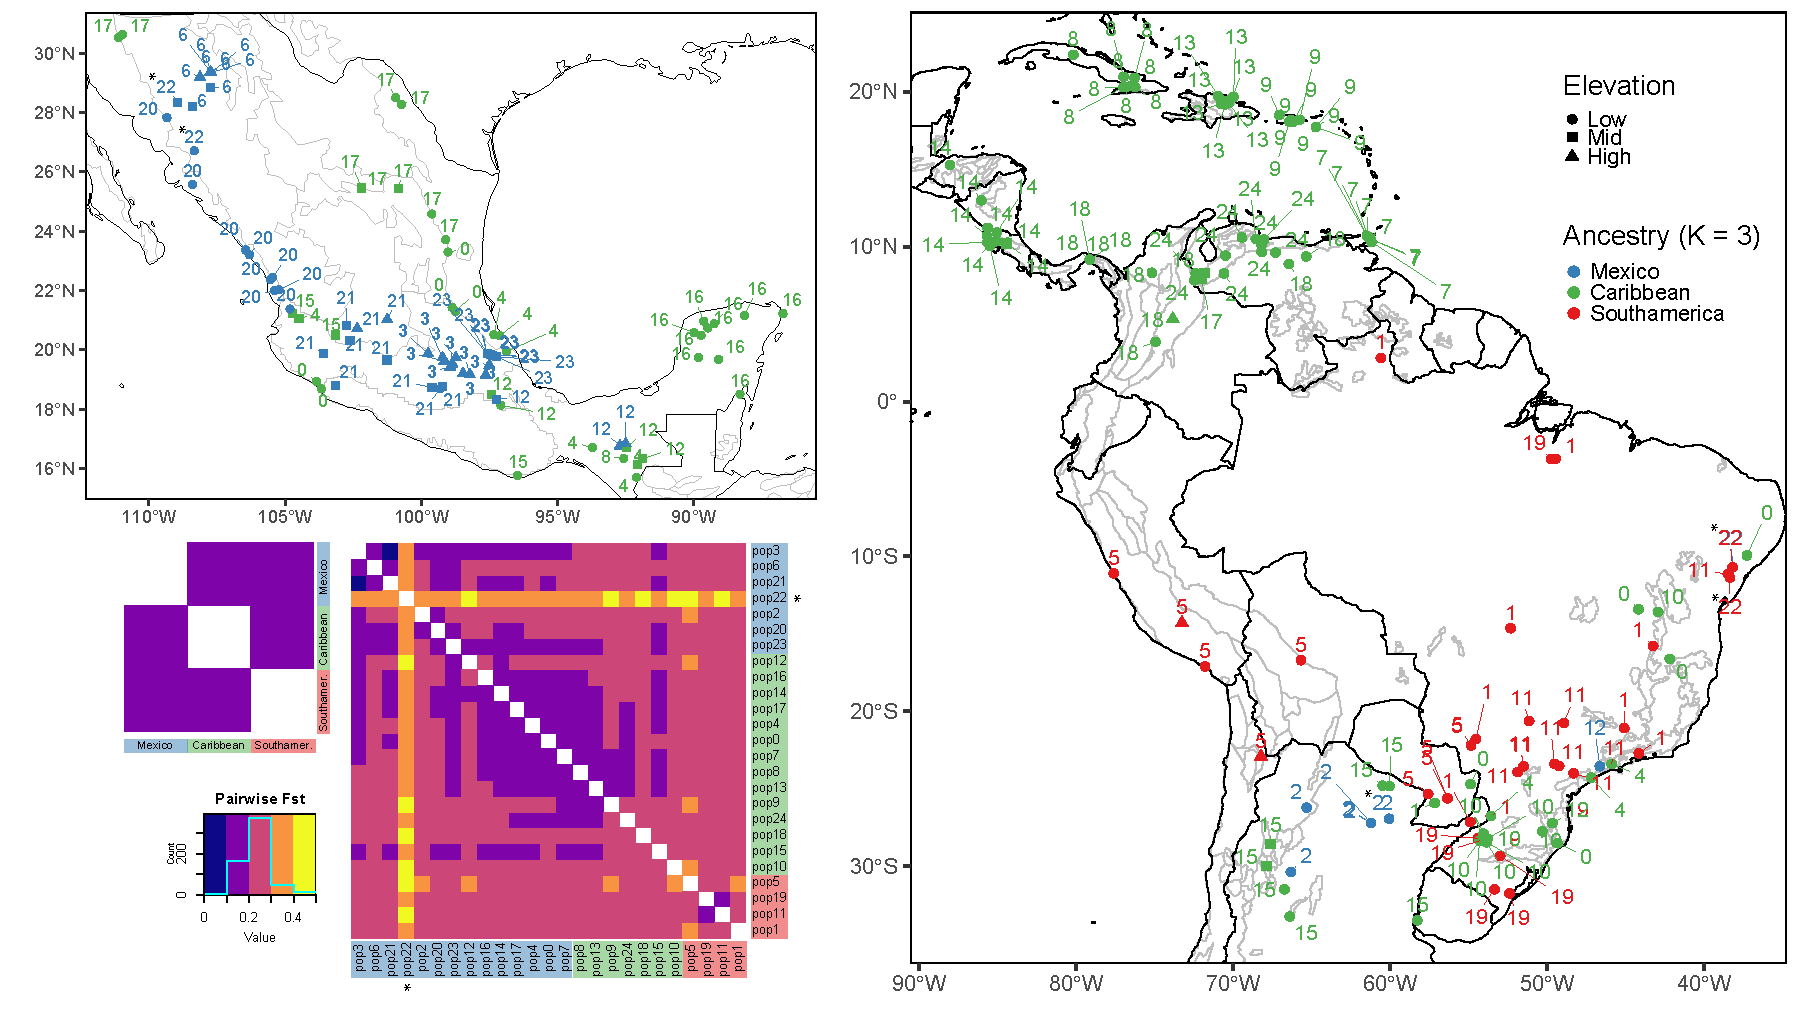
\includegraphics[width=\textwidth]{fig8.pdf}

% \caption{\color{Gray} \textbf{Population Map}.}

% \label{fig8} % \label works only AFTER \caption within figure environment

% \end{figure}

% \newpage

% \section*{Conclusion}

\nolinenumbers

\clearpage

\section*{Schedule}

\begin{figure}[!h]
   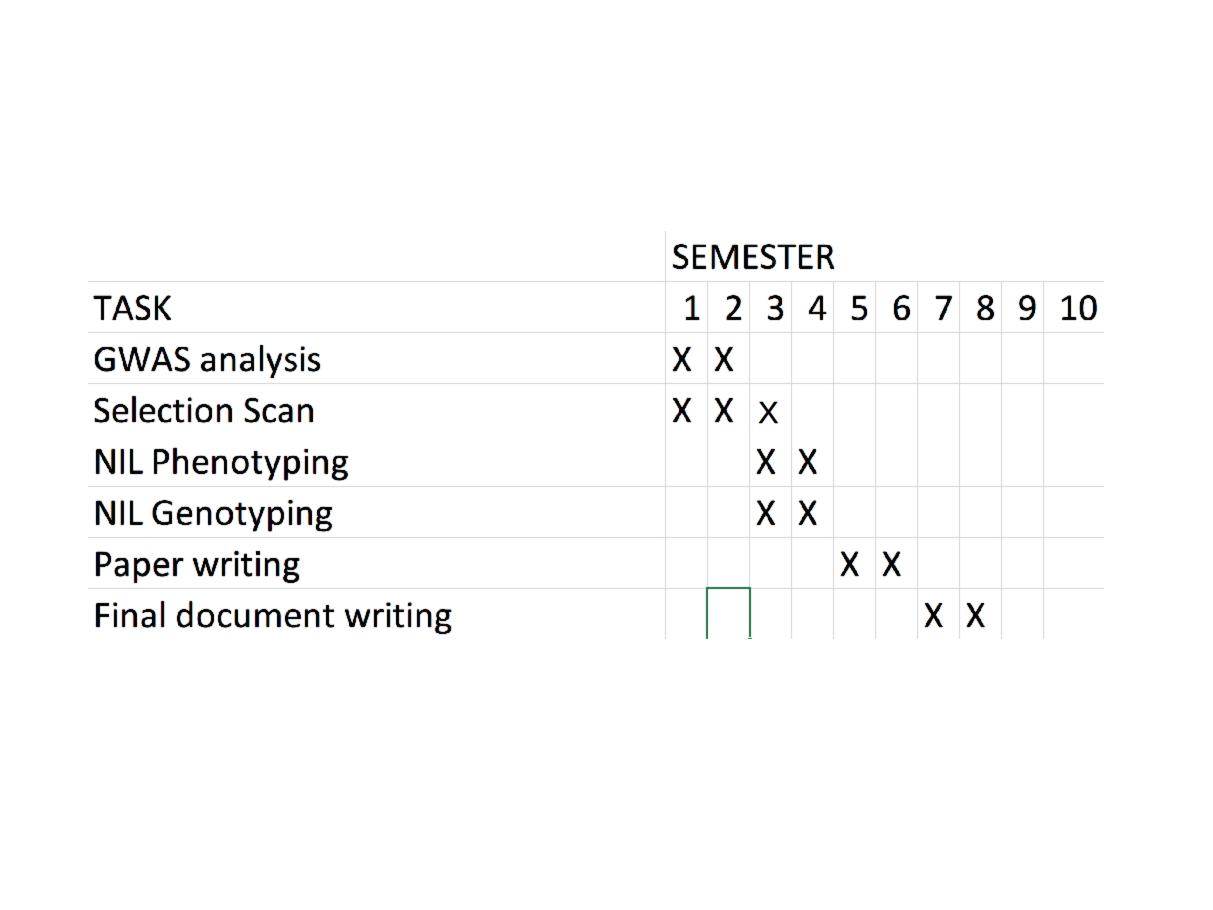
\includegraphics[width=\textwidth]{schedule.png}
   \caption{\textbf{Schedule}}
  \label{figSchedule} 
\end{figure} 

%This is where your bibliography is generated. Make sure that your .bib file is actually called library.bib
\bibliography{library}

%This defines the bibliographies style. Search online for a list of available styles.
\bibliographystyle{abbrv}

\end{document}

